% Options for packages loaded elsewhere
\PassOptionsToPackage{unicode}{hyperref}
\PassOptionsToPackage{hyphens}{url}
\PassOptionsToPackage{dvipsnames,svgnames,x11names}{xcolor}
%
\documentclass[
  super,
  preprint,
  3p]{elsarticle}

\usepackage{amsmath,amssymb}
\usepackage{setspace}
\usepackage{iftex}
\ifPDFTeX
  \usepackage[T1]{fontenc}
  \usepackage[utf8]{inputenc}
  \usepackage{textcomp} % provide euro and other symbols
\else % if luatex or xetex
  \usepackage{unicode-math}
  \defaultfontfeatures{Scale=MatchLowercase}
  \defaultfontfeatures[\rmfamily]{Ligatures=TeX,Scale=1}
\fi
\usepackage{lmodern}
\ifPDFTeX\else  
    % xetex/luatex font selection
    \setmainfont[]{Comic Sans MS}
\fi
% Use upquote if available, for straight quotes in verbatim environments
\IfFileExists{upquote.sty}{\usepackage{upquote}}{}
\IfFileExists{microtype.sty}{% use microtype if available
  \usepackage[]{microtype}
  \UseMicrotypeSet[protrusion]{basicmath} % disable protrusion for tt fonts
}{}
\makeatletter
\@ifundefined{KOMAClassName}{% if non-KOMA class
  \IfFileExists{parskip.sty}{%
    \usepackage{parskip}
  }{% else
    \setlength{\parindent}{0pt}
    \setlength{\parskip}{6pt plus 2pt minus 1pt}}
}{% if KOMA class
  \KOMAoptions{parskip=half}}
\makeatother
\usepackage{xcolor}
\setlength{\emergencystretch}{3em} % prevent overfull lines
\setcounter{secnumdepth}{5}
% Make \paragraph and \subparagraph free-standing
\makeatletter
\ifx\paragraph\undefined\else
  \let\oldparagraph\paragraph
  \renewcommand{\paragraph}{
    \@ifstar
      \xxxParagraphStar
      \xxxParagraphNoStar
  }
  \newcommand{\xxxParagraphStar}[1]{\oldparagraph*{#1}\mbox{}}
  \newcommand{\xxxParagraphNoStar}[1]{\oldparagraph{#1}\mbox{}}
\fi
\ifx\subparagraph\undefined\else
  \let\oldsubparagraph\subparagraph
  \renewcommand{\subparagraph}{
    \@ifstar
      \xxxSubParagraphStar
      \xxxSubParagraphNoStar
  }
  \newcommand{\xxxSubParagraphStar}[1]{\oldsubparagraph*{#1}\mbox{}}
  \newcommand{\xxxSubParagraphNoStar}[1]{\oldsubparagraph{#1}\mbox{}}
\fi
\makeatother

\usepackage{color}
\usepackage{fancyvrb}
\newcommand{\VerbBar}{|}
\newcommand{\VERB}{\Verb[commandchars=\\\{\}]}
\DefineVerbatimEnvironment{Highlighting}{Verbatim}{commandchars=\\\{\}}
% Add ',fontsize=\small' for more characters per line
\usepackage{framed}
\definecolor{shadecolor}{RGB}{241,243,245}
\newenvironment{Shaded}{\begin{snugshade}}{\end{snugshade}}
\newcommand{\AlertTok}[1]{\textcolor[rgb]{0.68,0.00,0.00}{#1}}
\newcommand{\AnnotationTok}[1]{\textcolor[rgb]{0.37,0.37,0.37}{#1}}
\newcommand{\AttributeTok}[1]{\textcolor[rgb]{0.40,0.45,0.13}{#1}}
\newcommand{\BaseNTok}[1]{\textcolor[rgb]{0.68,0.00,0.00}{#1}}
\newcommand{\BuiltInTok}[1]{\textcolor[rgb]{0.00,0.23,0.31}{#1}}
\newcommand{\CharTok}[1]{\textcolor[rgb]{0.13,0.47,0.30}{#1}}
\newcommand{\CommentTok}[1]{\textcolor[rgb]{0.37,0.37,0.37}{#1}}
\newcommand{\CommentVarTok}[1]{\textcolor[rgb]{0.37,0.37,0.37}{\textit{#1}}}
\newcommand{\ConstantTok}[1]{\textcolor[rgb]{0.56,0.35,0.01}{#1}}
\newcommand{\ControlFlowTok}[1]{\textcolor[rgb]{0.00,0.23,0.31}{\textbf{#1}}}
\newcommand{\DataTypeTok}[1]{\textcolor[rgb]{0.68,0.00,0.00}{#1}}
\newcommand{\DecValTok}[1]{\textcolor[rgb]{0.68,0.00,0.00}{#1}}
\newcommand{\DocumentationTok}[1]{\textcolor[rgb]{0.37,0.37,0.37}{\textit{#1}}}
\newcommand{\ErrorTok}[1]{\textcolor[rgb]{0.68,0.00,0.00}{#1}}
\newcommand{\ExtensionTok}[1]{\textcolor[rgb]{0.00,0.23,0.31}{#1}}
\newcommand{\FloatTok}[1]{\textcolor[rgb]{0.68,0.00,0.00}{#1}}
\newcommand{\FunctionTok}[1]{\textcolor[rgb]{0.28,0.35,0.67}{#1}}
\newcommand{\ImportTok}[1]{\textcolor[rgb]{0.00,0.46,0.62}{#1}}
\newcommand{\InformationTok}[1]{\textcolor[rgb]{0.37,0.37,0.37}{#1}}
\newcommand{\KeywordTok}[1]{\textcolor[rgb]{0.00,0.23,0.31}{\textbf{#1}}}
\newcommand{\NormalTok}[1]{\textcolor[rgb]{0.00,0.23,0.31}{#1}}
\newcommand{\OperatorTok}[1]{\textcolor[rgb]{0.37,0.37,0.37}{#1}}
\newcommand{\OtherTok}[1]{\textcolor[rgb]{0.00,0.23,0.31}{#1}}
\newcommand{\PreprocessorTok}[1]{\textcolor[rgb]{0.68,0.00,0.00}{#1}}
\newcommand{\RegionMarkerTok}[1]{\textcolor[rgb]{0.00,0.23,0.31}{#1}}
\newcommand{\SpecialCharTok}[1]{\textcolor[rgb]{0.37,0.37,0.37}{#1}}
\newcommand{\SpecialStringTok}[1]{\textcolor[rgb]{0.13,0.47,0.30}{#1}}
\newcommand{\StringTok}[1]{\textcolor[rgb]{0.13,0.47,0.30}{#1}}
\newcommand{\VariableTok}[1]{\textcolor[rgb]{0.07,0.07,0.07}{#1}}
\newcommand{\VerbatimStringTok}[1]{\textcolor[rgb]{0.13,0.47,0.30}{#1}}
\newcommand{\WarningTok}[1]{\textcolor[rgb]{0.37,0.37,0.37}{\textit{#1}}}

\providecommand{\tightlist}{%
  \setlength{\itemsep}{0pt}\setlength{\parskip}{0pt}}\usepackage{longtable,booktabs,array}
\usepackage{calc} % for calculating minipage widths
% Correct order of tables after \paragraph or \subparagraph
\usepackage{etoolbox}
\makeatletter
\patchcmd\longtable{\par}{\if@noskipsec\mbox{}\fi\par}{}{}
\makeatother
% Allow footnotes in longtable head/foot
\IfFileExists{footnotehyper.sty}{\usepackage{footnotehyper}}{\usepackage{footnote}}
\makesavenoteenv{longtable}
\usepackage{graphicx}
\makeatletter
\def\maxwidth{\ifdim\Gin@nat@width>\linewidth\linewidth\else\Gin@nat@width\fi}
\def\maxheight{\ifdim\Gin@nat@height>\textheight\textheight\else\Gin@nat@height\fi}
\makeatother
% Scale images if necessary, so that they will not overflow the page
% margins by default, and it is still possible to overwrite the defaults
% using explicit options in \includegraphics[width, height, ...]{}
\setkeys{Gin}{width=\maxwidth,height=\maxheight,keepaspectratio}
% Set default figure placement to htbp
\makeatletter
\def\fps@figure{htbp}
\makeatother

\usepackage{lineno}
\usepackage{caption}
\makeatletter
\@ifpackageloaded{caption}{}{\usepackage{caption}}
\AtBeginDocument{%
\ifdefined\contentsname
  \renewcommand*\contentsname{Table of contents}
\else
  \newcommand\contentsname{Table of contents}
\fi
\ifdefined\listfigurename
  \renewcommand*\listfigurename{List of Figures}
\else
  \newcommand\listfigurename{List of Figures}
\fi
\ifdefined\listtablename
  \renewcommand*\listtablename{List of Tables}
\else
  \newcommand\listtablename{List of Tables}
\fi
\ifdefined\figurename
  \renewcommand*\figurename{Figure}
\else
  \newcommand\figurename{Figure}
\fi
\ifdefined\tablename
  \renewcommand*\tablename{Table}
\else
  \newcommand\tablename{Table}
\fi
}
\@ifpackageloaded{float}{}{\usepackage{float}}
\floatstyle{ruled}
\@ifundefined{c@chapter}{\newfloat{codelisting}{h}{lop}}{\newfloat{codelisting}{h}{lop}[chapter]}
\floatname{codelisting}{Listing}
\newcommand*\listoflistings{\listof{codelisting}{List of Listings}}
\makeatother
\makeatletter
\makeatother
\makeatletter
\@ifpackageloaded{caption}{}{\usepackage{caption}}
\@ifpackageloaded{subcaption}{}{\usepackage{subcaption}}
\makeatother
\journal{Elsevier}

\ifLuaTeX
  \usepackage{selnolig}  % disable illegal ligatures
\fi
\usepackage[]{natbib}
\bibliographystyle{elsarticle-num}
\usepackage{bookmark}

\IfFileExists{xurl.sty}{\usepackage{xurl}}{} % add URL line breaks if available
\urlstyle{same} % disable monospaced font for URLs
\hypersetup{
  pdftitle={Evaluating the utility of graph similarity metrics in quantitative read-across: A tutorial},
  pdfauthor={Brett Hagan; Louis Groff; Imran Shah; Grace Patlewicz},
  pdfkeywords={Read-Across, Graph similarity, Graph kernels, Graph
convolutional networks (GCNs)},
  colorlinks=true,
  linkcolor={blue},
  filecolor={Maroon},
  citecolor={Blue},
  urlcolor={Blue},
  pdfcreator={LaTeX via pandoc}}


\setlength{\parindent}{6pt}
\begin{document}

\begin{frontmatter}
\title{Evaluating the utility of graph similarity metrics in
quantitative read-across: A tutorial}
\author[1,2]{Brett Hagan%
%
}

\author[2]{Louis Groff%
%
}

\author[2]{Imran Shah%
%
}

\author[]{Grace Patlewicz%
\corref{cor1}%
}
 \ead{patlewicz.grace@epa.gov} 

\affiliation[1]{organization={ORAU, Oak Ridge Associated
Universities},city={Oak Ridge},postcode={TN, USA},postcodesep={}}
\affiliation[2]{organization={Center for Computational Toxicology and
Exposure (CCTE), Office of Research and Development, US Environment
Protection Agency},addressline={109 TW Alexander Dr},city={Research
Triangle Park},postcode={NC 27711 USA},postcodesep={}}

\cortext[cor1]{Corresponding author}




        
\begin{abstract}
Read-across is a popular technique for filling data gaps for substances
lacking empirical data. The approach relies on identifying source
analogues with relevant data that are `similar' to a target substance.
Typically source analogues are identified on the basis of structural
similarity but the evaluation of their suitability for read-across
depends on other contexts of similarity including their physical
property information, chemical reactivity, bioactivity and metabolism.
Whilst quantifying structural similarity is well established, relying on
chemical fingerprints and using a similarity index such as Tanimoto to
limit the number of analogues returned, characterizing other aspects of
similarity objectively remains a challenge. The use of graph analytical
approaches has become an increasingly important tool that is employed in
a wide variety of domains. Since many different aspects of a substance
and its associated properties lend themselves to being represented by
graphs, using graph similarity offers new ways in which analogues could
be identified and evaluated for read-across purposes. This manuscript
considered the application of graph similarity measurements for
read-across. Several different methods were discussed, which have been
divided into three categories; graph kernel approaches, graph embedding
approaches, and deep learning (DL) approaches. Each approach was
described in brief together with a practical example to illustrate the
application for read-across purposes.
\end{abstract}





\begin{keyword}
    Read-Across \sep Graph similarity \sep Graph kernels \sep 
    Graph convolutional networks (GCNs)
\end{keyword}
\end{frontmatter}
    

\setstretch{1.5}
\section{Introduction}\label{introduction}

\subsection{Background to Read-Across}\label{sec-background}

An overwhelming and ever-increasing number of substances exist in
commerce, of which only a small proportion have undergone sufficient
toxicological evaluation. Assessing each chemical in turn presents a
significant and impractical challenge in terms of cost, animal welfare,
and resources \citep{nrc_toxicity_1984}. \emph{In vitro} and \emph{in
silico} approaches have the potential to play a large role in the
assessment of chemicals that lack empirical data. \emph{In silico}
approaches encompass (quantitative) structure activity relationships
((Q)SAR) as well as read-across (RAx), both of which relate chemical
structural properties to (eco)toxicological or physical property
endpoints. RAx is probably the most commonly used data gap filling
technique for regulatory purposes, notably it is cited as the most
commonly used adaptation to address information requirements under the
European Union's Registration Evaluation and Authorisation of Chemicals
(REACH) regulation \citep{eu_regulation_2006, macmillan_last_2024}. In
brief, RAx describes the method for filling a data gap whereby a
substance with existing data (termed the `source analogue') is used to
make a prediction of the same property for a `target' substance with
limited available empirical data. These predictions operate on the
assumption that the source and target substances are `similar' in some
context with relevant information pertaining to a specific outcome
\citep{enoch_chemical_2010, oecd_guidance_2014}. Key to this approach is
the characterization of similarity. Although structural similarity is
typically the most common approach used to identify candidate source
analogues, other similarity contexts namely similarity in
physicochemical properties, metabolism, toxicokinetics, chemical
reactivity, bioactivity and toxicological profile also play a
significant role in justifying those source analogues for read-across.
This is evident in the assessment frameworks that have been published
such as the European Chemicals Agency's Read-Across Assessment Framework
(RAAF) \citep{european_chemicals_agency_read-across_2017} as well as the
analogue workflow underpinning the US Environmental Protection Agency's
Provisional Peer Review Toxicity Values (PPRTV)
\citep{wang_application_2012}. For example, metabolic similarity
considers the similarity of transformation pathways as determined in
experimental studies or the commonality of metabolites formed.
Physicochemical similarity compares certain physical property
information such as LogKow, melting point, boiling point etc. of source
analogues relative to the target chemical to determine whether physical
form and partitioning are likely to be the same. Similarity in toxicity
assesses available empirical data to identify whether target organs
impacted are the same and whether the potencies are comparable or follow
a specific trend. Such similarity context assessments are largely
qualitative and heavily reliant on expert judgement in concert with
empirical data \citep{patlewicz_building_2015}. This does result in
challenges in terms of reproducibility, scalability and acceptance for
regulatory purposes \citep{shah_systematically_2016}. Indeed, RAx as a
technique has been in use for well over 20 years, but hesitation
regarding the adoption of the approach for certain regulatory contexts
(e.g.~risk assessment) or within specific jurisdictions remains
\citep{patlewicz_towards_2023}. Thus, progress towards approaches that
may increase confidence in and reduce the levels of inherent uncertainty
in RAx predictions remain of vital importance in the ongoing adoption of
RAx for regulatory purposes. Significant effort has been directed
towards the evaluation of confidence in analogue selection in RAx across
a wide range of studies
\citep{patlewicz_building_2015, blackburn_framework_2014, schultz_assessing_2019, wu_framework_2010, patlewicz_navigating_2018}.
Several studies have aimed to define frameworks for characterizing
uncertainty
\citep{schultz_assessing_2019, schultz_strategy_2015, blackburn_framework_2014, patlewicz_navigating_2018},
others have demonstrated how high-throughput screening data can be
helpful in substantiating RAx justifications
\citep{escher_towards_2019, patlewicz_navigating_2018, rovida_nam-supported_2021}
by providing some evidence of mechanistic or biological similarity. The
European Chemicals Agency (ECHA) have developed a read-across assessment
framework to address this need
\citep{european_chemicals_agency_read-across_2017} whereas the
Organisation of Economic and Co-operative Development (OECD) have been
facilitating the development of case studies with the aim of updating
existing grouping technical guidance \citep{oecd_guidance_2014} with one
focus being on reducing read-across uncertainties \citep{OECD_IATA}.

In our own studies, Generalized Read-Across (GenRA)
\citep{shah_systematically_2016, patlewicz_towards_2023} was created
with the goals of quantifying performance and uncertainty by
establishing consistent performance baselines and quantifying the
contribution of different similarity contexts play in identifying of
source analogues or making toxicity predictions. Within GenRA (and RAx
in general), approaches typically use structural information such as
chemical fingerprints to identify candidate source analogues. Many
software tools exist that facilitate this type of analogue searching,
including the similarity searches within the EPA CompTox Chemicals
Dashboard \citep{williams_comptox_2017},
\href{https://pubchem.ncbi.nlm.nih.gov/}{PubChem}, as well as the many
functionalities within the OECD Toolbox (qsartoolbox.org)
\citep{schultz_oecd_2018}. There have been a number of efforts to study
additional sources of information to perform RAx, including the use of
physiochemical \citep{helman_extending_2018}, mechanistic
\citep{escher_towards_2019}, bioactivity
\citep{shah_systematically_2016, escher_towards_2019}, and metabolic
data \citep{lester_quantifying_2023, gadaleta_automated_2020}. Within
GenRA, research has continued to systematically evaluate the impact that
different types of similarity play in read-across for the prediction of
\emph{in vivo} toxicity
outcomes\citep{patlewicz_systematic_2024, tate_repeat-dose_2021, helman_extending_2018, nelms_mechanistic_2018, boyce_comparing_2022}
along with implementing the insights learned into the GenRA
(www.comptox.gov/genra) web application
\citep{patlewicz_towards_2023, shah_genra_2024}.

\subsection{Source analogue
identification}\label{source-analogue-identification}

As mentioned in Section~\ref{sec-background}, there are a number of
software tools that facilitate the identification of source analogues.
Most of these use structural similarity as a basis to return analogues.
This can be done in two main ways - either by a descriptor-based
similarity calculation or a substructure-based assessment
\citep{kunimoto_maximum_2016}. In practice, this means that a software
tool contains a large database (or dataset) of chemical substances which
serves as a source analogue inventory. To identify analogues, a search
query is then performed using the target substance of interest to return
candidate analogues. In a substructure-based approach, a determination
of the substructures shared with the target substance are made or
matched molecular pairs \citep{oboyle_using_2014, noauthor_matched_2021}
are generated to identify common core structures that are distinguished
at a given site. Such substructure-based calculations are binary -
either the target and source analogues share a pre-defined substructure
or not, therefore no adjustable threshold exists to tune the returned
set of candidate analogues. On the otherhand, the hits returned are
often chemical intuitive and interpretable.

In a descriptor-based approach, the key considerations are how the
substances forming the source inventory are represented numerically and
what metric is used to quantify a specific threshold of similarity.
Source analogues can be characterized by 1D, 2D or 3D representations of
structures or hybrids of these. For the aforementioned tools, 1D binary
chemical fingerprints are frequently used for practical efficiency
especially when a source inventory contains large numbers of substances
e.g.~1 million substances. A target substance will then be converted
into the same chemical fingerprint representation and a query based on
pairwise similarities will return a number of candidates based on the
similarity threshold set. The similarity threshold is a quantitative
measure between 0 and 1 that summarizes the commonality in structure
based on the presence and absence of particular chemical fingerprints.
By far, the most common similarity index that is used in the Tanimoto
(Jaccard) index \citep{bajusz_why_2015} though there are a number of
other similarity indices that can also be used
\citep{bajusz_why_2015, floris_generalizable_2014}. There are several
types of chemical fingerprints, one of the most popular is the Morgan
fingerprint \citep{rogers_extended-connectivity_2010}, also known as the
extended connectivity fingerprint (ECFP4).This perceives the presence of
specific circular fragments around each atom in a molecule. It relies on
the fragmentation of a molecule into circular fragments with each atom
encoded as atom types. Other fingerprints are termed key or dictionary
fingerprints where there is a defined fixed set of substructural
features representing molecular characteristics. MACCS (Molecular Access
System by Molecular Design Limited) \citep{durant_reoptimization_2002}
and ChemoType ToxPrints \citep{yang_new_2015} are examples of these.
Atom pairs is another example where an algortihm of atom typing is
performed such that certain values for each atom of a molecule is
computed \citep{carhart_atom_1985}. In each case, the fingerprint is
represented as a bit string or binary vector that can be used to search
for source analogues.

Chemical fingerprints have proved useful for fast similarity comparisons
as well as inputs into development of QSARs for different activity
outcomes in particular toxicity endpoints. Regardless of the fingerprint
type, there are always limitations in how a chemical may be represented
to capture the aspects important for toxicity prediction. For example,
circular fingerprints are typically poor at perceiving global features
of a molecule (e.g.~size or shape) and may fail to discriminate between
subtle changes between 2 small molecules. In any case, chemical
fingerprints represent a simplified representation of a chemical that
may be insufficient to resolve differences in toxicity outcomes.

Consideration of the other similarity contexts offers a means of
addressing this shortcoming although leveraging the inherent
representation of a chemical structure as a graph, with atoms as nodes
and bonds as edges, offers alternative opportunities to eliminate the
need for precomputed features and fingerprints.

\subsection{Graph Terminology}\label{graph-terminology}

For context, a few of the pertinent terms/definitions associated with
graphs are described. A graph \[ G(V, E) \] is a visual representation
of a collection of nodes (also called vertices depending on domain) and
edges that connect these nodes providing a structure to represent
entities and their relationships. There are three main types of edges
that are typically found in a graph: undirected edges, directed edges
and weighted edges.

Figure~\ref{fig-gg} provides an example of an undirected graph with 5
nodes and 5 edges and the corresponding directed graph.

\begin{figure}

\begin{minipage}{\linewidth}

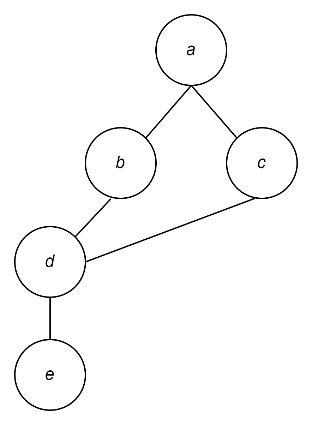
\includegraphics[width=0.3\textwidth,height=\textheight]{fig-gp.png}

\end{minipage}%

\caption{\label{fig-gg}Undirected and directed graph with 5 nodes and 5
edges.}

\end{figure}%

Undirected edges are those which identify a connection between nodes but
without a given ``flow''. Directed edges are those where is a clear
direction between nodes e.g.~within a metabolic graph where a parent
chemical transforms into a metabolite. Weighted edges can occur in both
directed or undirected edges to depict some quantitative value e.g.~the
rate of disappearance of parent chemical to its corresponding
metabolite.

The neighborhood of a node N(v) is the set of all nodes adjacent to v.
In Figure~\ref{fig-gg}, the neighborhood of node d would be expressed as
N(d) = {[}b,c,e{]}. A \emph{walk} comprises a sequence of edges and
nodes, whereas a \emph{path} is a walk with no repeating nodes visited.
In Figure~\ref{fig-path}, the sequence of nodes {[}a,b,d{]} is both a
walk and a path in graph G.

\begin{figure}

\centering{

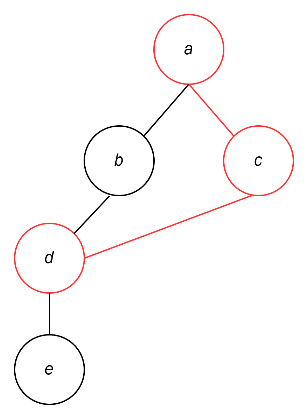
\includegraphics[width=0.3\textwidth,height=\textheight]{fig-path.png}

}

\caption{\label{fig-path}The sequence of nodes {[}a,c,d{]} is both a
walk and a path on G since there are no repeating nodes in the
sequence.}

\end{figure}%

Two graphs are isomorphic if there is a structure that preserves a
one-to-one correspondence between the nodes and edges. In other words,
if the two graphs differ only by the names of the edges and nodes but
are otherwise structurally equivalent, they are said to be isomorphic.

Graph analytical approaches have been used in a number of different
domains including biology (to model biological systems such as
protein-protein interaction networks or metabolic networks), social
sciences (to study complex social networks), computer science (to model
malware, botnet, and anomaly detection), and engineering (to model
complex systems such as transportation networks, electrical power grids)
\citep{RN20}.

\subsection{Topological indices}\label{topological-indices}

Considering chemicals as graphs is not a novel concept. In fact, a wide
variety of chemical properties and processes have been modelled using
information derived from molecular graphs. Topological indices which
have been in use for more than 45 years are algebraic invariants of
hydrogen depleted molecular graphs which represent the topology of a
molecule. There are hundreds of topological indices but the majority can
be broadly categorized into 5 main types namely: degree-based indices,
distance-based indices, count-based indices, eigenvalue-based indices
and information-theoretic indices \citep{balaban_topological_1983}.
Degree indices are based on the degree of the nodes in the graph. The
Zagreb Index is based on the degrees of the nodes focusing on the sum of
squares or products of node degrees whereas the Randic Index is defined
by the sum of the inverse of the square roots of the degrees of adjacent
nodes. The most common distance based index is the Wiener Index, which
represents the sum of the shortest-path distances between all pairs of
nodes in the graph. Count based indices include the Hosoya Index which
counts the number of matching sets in the graph. Eigenvalue based
indices include the Estrada index which is the sum of the exponential of
the eigenvalues of the adjacency matrix. Finally information-theoretic
indices use concepts from information theory to quantify the
distribution of certain properties within the graph. The Shannon entropy
measures the diversity in the distributon of node degrees. Topological
indices have been widely and successfully applied to the quantitative
correlation of many different molecular properties such as boiling
point, chemical reactivity as well as biological activity
\citep{roy_use_2017}. Topological indices summarize a chemical into a
single number or set of numbers. Although the indices have been used in
many QSAR studies, one of their main shortcomings was a perceived lack
of interpretability \citep{todeschini_chemical_1992}.

\subsection{Graph Similarity}\label{graph-similarity}

Graph similarity is a well-studied problem with investigations being
focused upon direct operations that examine structural properties such
as graph edit distance, graph isomorphism and maximum common subgraph
matching approaches
\citep{ullmann_algorithm_1976, pelillo_replicator_1999, melnik_similarity_2002, jeh_simrank_2002, zager_graph_2008, koutra_algorithms_2011, chartrand_graph_1998}.

\subsubsection{Graph edit distances using Reduced
graphs}\label{graph-edit-distances-using-reduced-graphs}

Reduced graphs provide a summarised representation of a chemical
structure that are produced by collapsing connected atoms into single
nodes and forming edges between the nodes in accordance with bonds in
the original structure. Reduced graphs have been used in a variety of
applications in chemoinformatics ranging from the representation and
search of Markush structures to the identification of structure-activity
relationships (SARs). There are a number of different graph reduction
schemes though each has been devised to address a different purpose
\citep{gillet_similarity_2003, birchall_reduced_2011, birchall_training_2006}.
Graph reduction schemes have been developed for similarity searching
often with the objective of identifying substances with similarity in
activity. Various methods have also been developed to quantify the
similarity between reduced graphs from fingerprint approaches, graph
matching as well as an edit distance method. The edit distance approach
quantifies the degree of similarity of 2 reduced graphs based on the
number and type of operations needed to convert one graph to the other.
One benefit of the edit distance method is the ability to assign
different weights to different operations - useful when deriving
activity specific weights as evidenced in Birchall et al.
\citep{birchall_training_2006}. However, graph edit distance are
computationally expensive unless approximation algortihms are used
particularly for larger graphs. Garcia-Hernandez et al.~employed graph
edit distances to reduced graph representations to estimate the
bioactivity of a chemical on the basis of the bioactivity of similar
compounds and found better performance than the array
representation-based approaches they compared against \citep{RN25}.

\subsubsection{Graph isomorphism}\label{graph-isomorphism}

Several foundational questions of chemical similarity analysis have been
framed as graph comparison problems; chemical equivalence may be modeled
as a graph isomorphism task. Searching for a specific substructure
(e.g.~a benzene ring) within a chemical has been modeled as a subgraph
isomorphism task. The enumeration of possible chemical structures is
closely related to graph enumeration \citep{RN22}.

\subsubsection{Maximum common subgraph}\label{maximum-common-subgraph}

A common need in cheminformatics to the ability to align pairs of
molecules together to make a determination of the degree of structural
overlap. This is useful when exploring SARs, predicting bioactivity of
substances or identifying chemical reaction sites. The degree of overlap
between a pair of chemicals can be achieved using maximum common
subgraph isomorphism algorithms
\citep{duesbury_maximum_2017, raymond_maximum_2002}. In cheminformatics,
maximum common subgraph isomorphism is usually referred to as
identifying the maximum common substructure (MCS). As put by A Dalke,
``given two structures, the MCS is the largest substructure common to
both''. Maximum could be interpreted to imply the maximum number of
atoms, number of bonds, number of cycles or even some physical property.
There are also variations in how atom and bond equivalency might be
defined. However the most common MCS is where all atoms are the same if
the element numbers are the same and the bonds are of the same type (see
\url{http://dalkescientific.com/writings/diary/archive/2012/05/12/mcs_background.html}).
There are a range of algorithms that can determine the MCS between pairs
of chemicals. Some algorithms and perhaps the most prevalent work on the
basis of identifing cliques or maximal cliques. Examples include the
Bron-Kerbosch algorithm \citep{bron_algorithm_1973} which reports all of
the maximal cliques found. A clique is a set of nodes in a graph such
that each node is connected to each and every other node, with a maximal
clique in a graph being one that is not contained within another large
clique. TOPSIM \citep{durand_efficient_1999} is another algorithm
designed to find the Maximum Common Edge Subgraph (MCES) between two
graphs. The Maximum Common Edge Subgraph is similar to the Maximum
Common Subgraph (MCS) problem but focuses on finding the largest
subgraph that has the maximum number of edges in common between the two
graphs. In this case, the algorithm converts labeled graph
representations of two molecules into a compatibility graph. Then a
modified maximal clique algorithm is used to find the maximal clique
which represents the largest common substructure (excluding common
isolated atoms) for the two molecules. A maximal common substructure is
obtained by combining the largest common substructure and the common
isolated atoms. The size of a maximal common substructure is then used
to define both a molecular similarity index and a topological distance
for two molecules. Other types of algorithms include subgraph
enumeration algorithms which involve enumerating all connected subgraphs
common to the two graphs that are being compared and then returning the
largest subgraph. Raymond and Willett (2002) reviewed the main solutions
for pairwise MCS \citep{raymond_maximum_2002} including multiple MCS
\citep{dalke_fmcs_2013}.

More recent efforts to evaluate graph similarity include graph kernel
methods, graph embedding methods, and deep learning (DL) methods (which
can be considered to be a subset of graph embedding approaches in
general). Graph kernel methods directly calculate a similarity score
between two graphs based on their structural properties. Graph embedding
methods transform graphs into numerical representations (vectors) that
can be compared using standard distance metrics. Deep learning methods,
a subset of graph embedding, learn these numerical representations
automatically using neural networks.

\subsubsection{Graph Kernels}\label{graph-kernels}

Graph kernels were first introduced as a way to compare complex
structures like graphs based on a concept from Haussler's work on
kernels for discrete structures \citep{kondor_diffusion_2002}. The term
``graph kernels'' soon emerged to describe methods specifically for
comparing graphs \citep{RN27, RN45, scholkopf_fast_2007}. The core idea
behind graph kernels is to break down a graph into smaller components,
called substructures. These substructures are then used to create
feature vectors, which characterize the graph. By comparing these
feature vectors, it is possible to measure how similar two graphs are.
The inner products of the feature vectors can be efficiently computed to
produce a similarity score between the graphs. The key to graph kernels
lies in how the graph is decomposed. One simple approach is to count how
many node labels are shared between graphs and computing the inner
products of these label counts to produce a similarity score
\citep{kriege_survey_2020}. Figure~\ref{fig-count} provides an example
of counting node labels.

\begin{figure}

\centering{

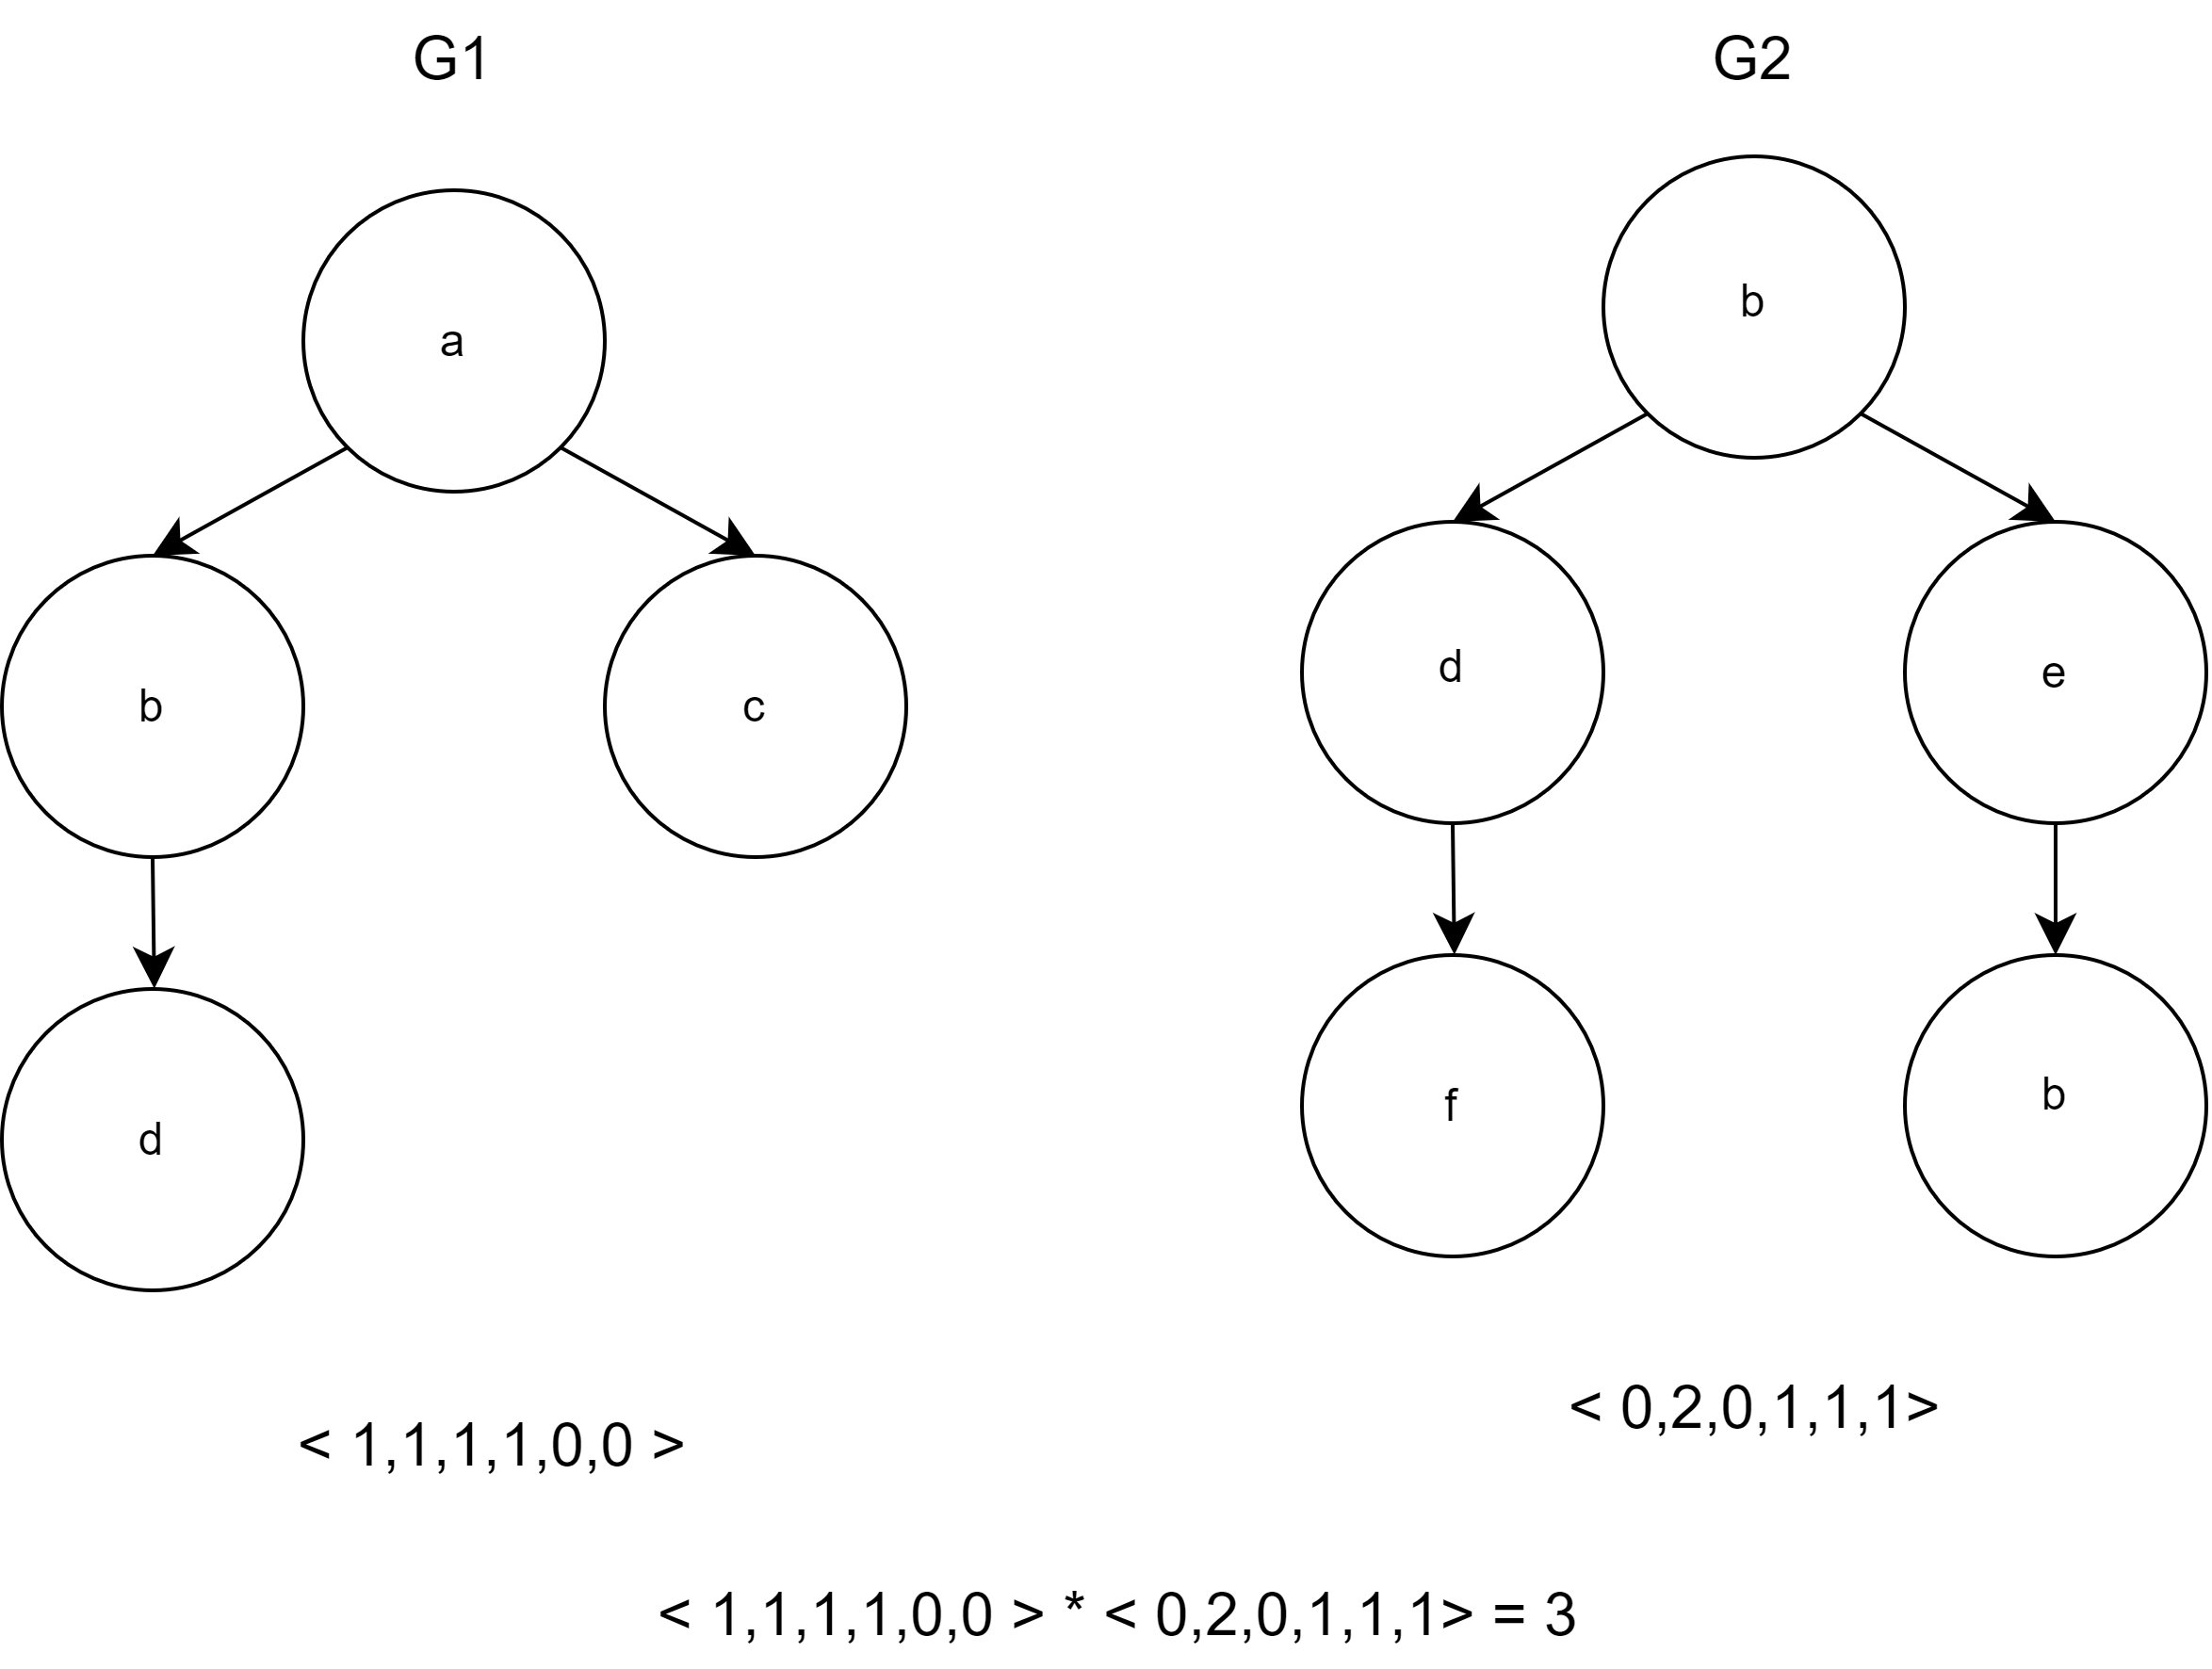
\includegraphics[width=1\textwidth,height=\textheight]{fig-count.png}

}

\caption{\label{fig-count}Graph kernel counting node labels.The feature
vectors for both graphs are constructed by counting the numbers of node
labels in each graph. A similarity score is then obtained by computing
the inner products of the feature vectors.}

\end{figure}%

There are many different ways to decompose a graph in order to compare
them. One approach is through Random walk kernels. This method involves
taking random paths through the graph and counting how often each path
occurs in each graph \citep{gartner_survey_2003}. Shortest path kernels
aim to find the shortest paths between labeled nodes (atoms) in each
graph and using these to construct feature vectors \citep{RN30}. A more
advanced method builds on the Weisfeiler-Lehman (WL) graph isomorphism
heuristic that was introduced by Shervashidze in 2011; known as the WL
subtree kernel \citep{RN46}. The WL isomorphism heuristic works by
iteratively updating the labels of each atom based on the labels of its
neighboring atoms. Over several iterations, this process captures more
detailed substructures within the molecule. If at any point the labels
of the nodes in the graphs do not match, the algorithm is terminated as
the two graphs can not be isomorphic. The WL subtree kernel then uses
these refined labels to compare different molecular graphs. This method
is particularly powerful and has been found to be closely related to
operations used in graph neural networks. Figure~\ref{fig-wl} shows an
example iteration of the kernel between two graphs.

\begin{figure}

\centering{

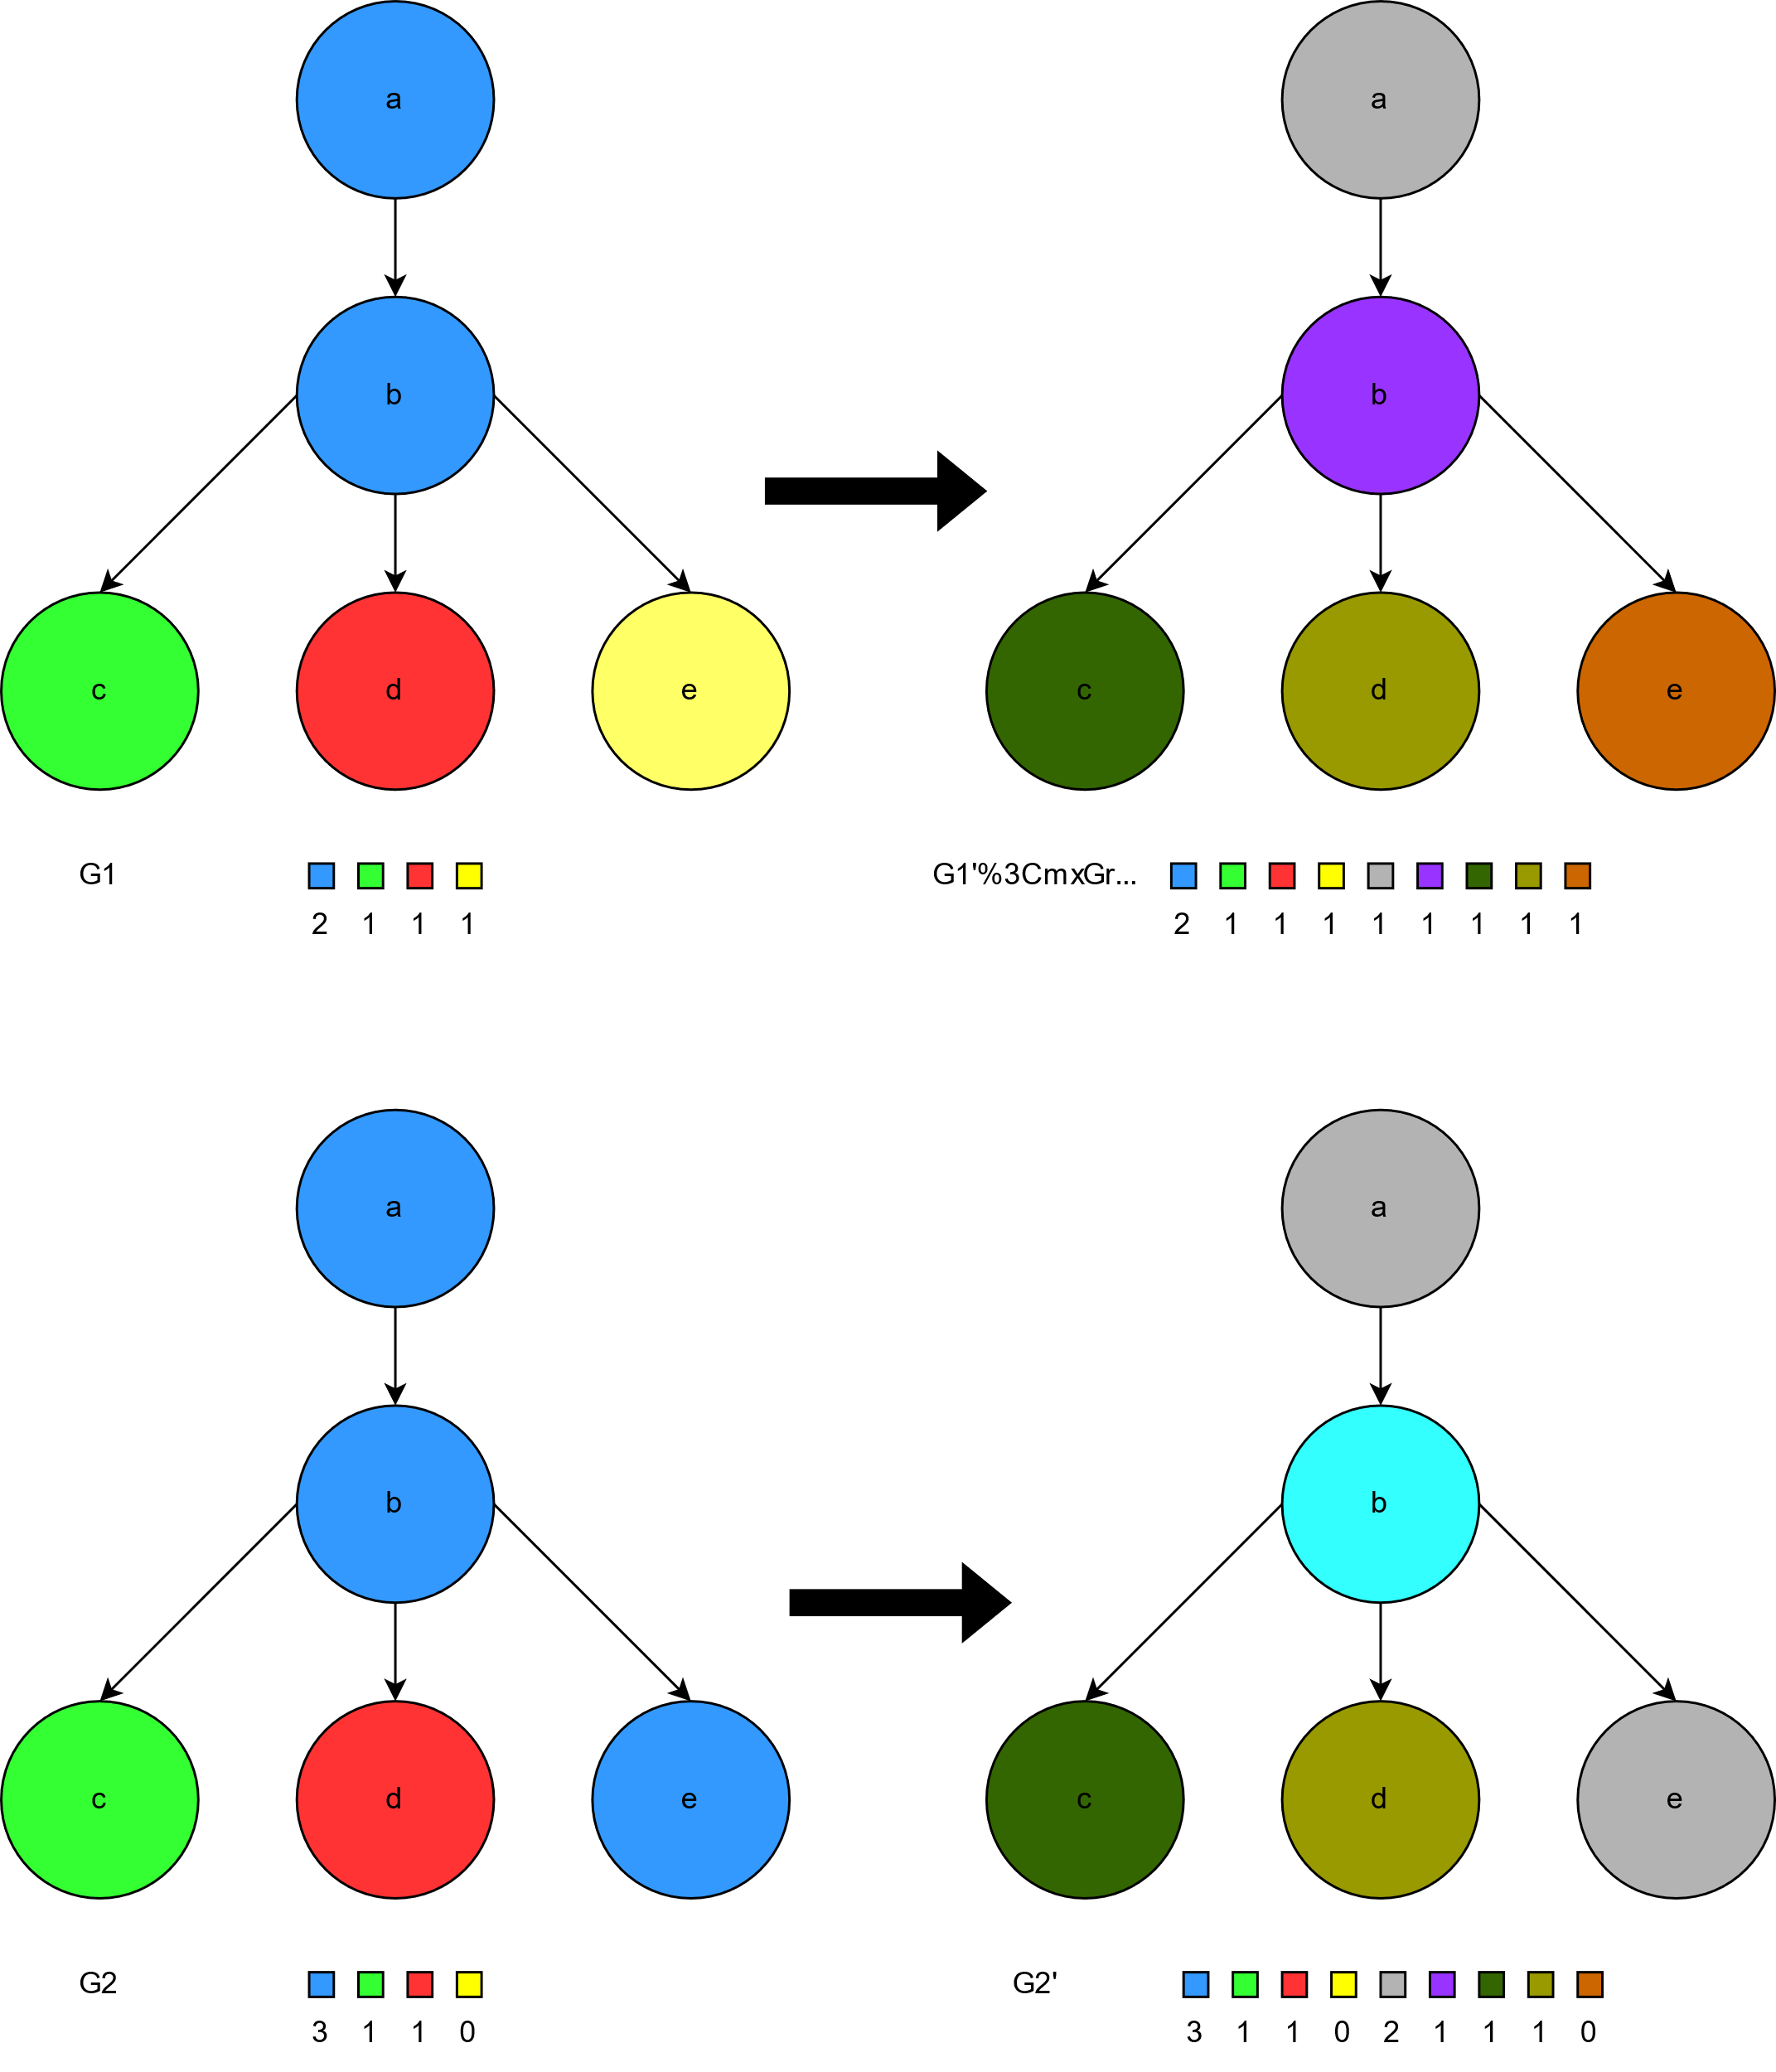
\includegraphics[width=0.5\textwidth,height=\textheight]{wl.png}

}

\caption{\label{fig-wl}One iteration of the WL kernel. Feature vectors
initially consist of counts of original atom labels. At each iteration,
new labels (colors) are created for each atoms by considering the labels
of its neighbors. Nodes a in both G1' and G2' are labeled gray as they
were both adjacent to a single blue label in the previous iteration,
whereas nodes e in G1' and G2' are assigned different labels due to the
differences in their neighboring node labels. The feature vectors
consist of counts of the original and newly created node labels as
iteration continues until a defined limit or convergence is reached. The
inner products are computed to obtain a similarity score.}

\end{figure}%

\subsubsection{Graph Embeddings}\label{sec-graphembed}

While there are numerous advantageous qualities to graph
representations, there are also some inherent drawbacks to consider.
Graphs are highly dimensional, heterogenous data, the analysis of which
often involves large amounts of computational complexity and memory
requirements \citep{cai_comprehensive_2018}. Additionally, many tasks
are ill suited for the direct use of graph data. Visualization of sets
of graphs, or use as input into established machine learning techniques
such as clustering or classification require lower dimensional,
structured representations of data. To accomplish these goals, graph
embedding techniques may be employed to create lower dimensional
representations of graph data that retain as much topological and label
(or feature) information as possible. Highly informed graph embeddings
can also provide a sense of similarity between graphs, being that, for
sufficiently informative embeddings, highly similar graphs will have
highly similar graph embeddings, with little distance between their
embeddings in a latent space when compared to dissimilar graphs.
Embeddings can refer to both node embeddings, in which a graph is given
as input and individual vectorized embeddings for each node in the graph
are returned, or to whole graph embeddings, in which a single vectorized
representation of the entire graph is returned.

A number of different methods exist that are capable of creating graph
embeddings which can be broadly divided into two categories: node
embeddings, and whole graph embeddings. \textbf{Node embeddings} map
individual nodes in a graph to numerical vectors, capturing node
characteristics and relationships. \textbf{Graph embeddings} represent
the entire graph as a single vector, often by combining node embeddings
or using other methods, enabling comparisons between graphs.There are a
variety of different approaches to either task, with well established
taxonomies in literature dividing them into three distinct categories;
matrix factorization methods, random walk based methods, and neural
network methods, with substantial areas of overlap between the three
\citep{xu_understanding_2021, goyal_graph_2018}.

Matrix factorization techniques were the earliest studied, beginning
with the multi-dimensional scaling (MDS) that decomposed adjacency
matrices \citep{RN34}. Other factorization methods operate on graph
proximity (distance matrices) or graph Laplacian matrices
\citep{RN35, RN36}. Although factorization methods are the most
well-established and theoretically understood, they often scale poorly
\citep{xu_understanding_2020}. Random walk based embeddings
\citep{perozzi_deepwalk_2014} later emerged based upon word and document
embedding methodologies such as Word2Vec, adopting the skip-gram neural
network model used to create word embeddings to the graph context. The
skip-gram model is a simple single hidden layer neural network (see
Figure~\ref{fig-skip}) that is trained to predict the probabilities for
each word in a given vocabulary to appear near in sequence to a given
target word. The network is trained, and the weights of the trained
network are exploited as vectorized word embeddings, with the underlying
intuition being that words that often appear in similar contexts are
likely highly similar in some context \citep{mikolov_efficient_2013}.

\begin{figure}

\centering{

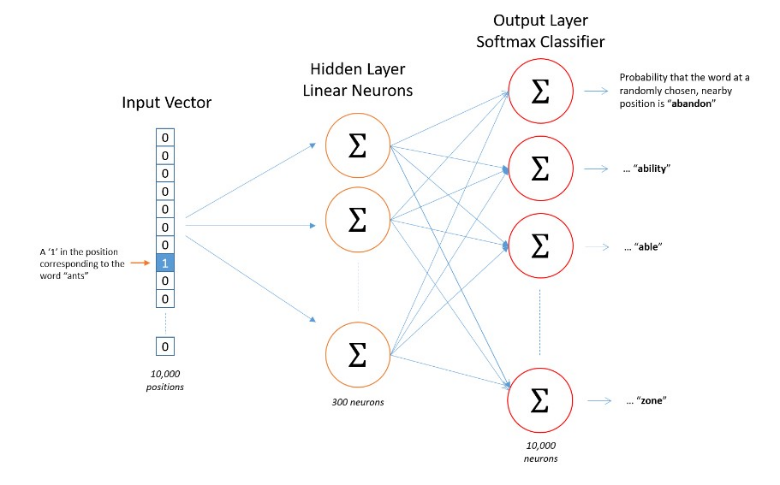
\includegraphics{survey_skip_gram_figure.png}

}

\caption{\label{fig-skip}Skip gram model for Word2Vec word embeddings. A
one hidden layer neural network is trained to determine the
probabilities for each word in a vocabulary of appearing near in
sequence to a given target word. The target word is given as a one-hot
encoded input, and after training via backpropagation over a number of
epochs, the hidden weights of the network are used as embedded vector
representations of words.}

\end{figure}%

DeepWalk adapted the SkipGram approach to a graph setting
\citep{perozzi_deepwalk_2014} for node embedding. Words are analogous to
nodes in the graph, the sequences of words (a ``context'') are analogous
to random walks across node neighborhoods, and the vocabulary of words
is analogous to all nodes in the graph. Node2Vec iterated upon DeepWalk
with the introduction of parameters to control the length and freedom of
the random walk operations \citep{RN40}. Graph2Vec iterated upon
Node2Vec to allow for skip-gram based whole graph embeddings based off
rooted subgraphs analogous to words in Word2Vec
\citep{narayanan_graph2vec_2017}. GL2Vec improved upon Graph2Vec in
classification tasks by incorporating information gleaned from a line
graph representation, better allowing for the capture of structural
information \citep{RN42}. Research has shown that more complicated
approaches to graph embeddings may not necessarily result in better
performance. The LDP (Local Degree Profile) embedding method was
introduced in 2019 and showed comparable performance to more
sophisticated embeddings methods while only considering the degree
information of nodes in a graphs without considering any label
information whatsoever \citep{RN32}.

\subsubsection{Deep Learning Embeddings}\label{deep-learning-embeddings}

Inspired by widespread success of various deep learning approaches such
as convolutional neural networks (CNNs), graph neural networks (GNNs)
were introduced in 2008 with the goal of extending existing neural
network models for processing graph structured data
\citep{scarselli_graph_2009}. Early approaches focused mainly on
iteratively learning individual node representations through propagation
of neighboring node information. Taking inspiration from the concept of
convolutional operations on structured data for image processing tasks,
graph convolutional networks (GCNs) were defined. The GCN model
introduced by Kipf and Welling in 2016 \citep{kipf_2017} operates on a
graph or set of graphs via convolutions and activations. Each training
epoch consists of two primary operations, an aggregation of neighborhood
node information, followed by an update that uses the aggregated
information to update individual node embeddings (see
Figure~\ref{fig-gcn-concept}). The particulars of each operation are
dependent upon the layer type used. The GCN model generates node
embeddings, but whole graph embeddings can be easily generated by the
addition of a pooling or ``readout'' layer that aggregates the
individual node's information by some method such as taking the mean,
maximum, or minimum, and producing a whole graph embedding. Fully
connected linear layers can be stacked onto the end of a GCN model to
create end-to-end pipelines for ML tasks on graphs such as
classification or regression. For whole graph classification, a number
of linear layers and activation functions can be added to a network
following the readout layer and the model is trained in a supervised
manner to classify given graphs. A loss function such as cross-entropy
or mean squared error is calculated and model weights adjusted through
backpropagation. In addition to the use of a GCN in an end-to-end
classification setting, this model can also be used to derive whole
graph embeddings that are informed on some classification outcome. To do
this, labeled graph data are used as an input. A GCN graph
classification model is trained over a number of epochs, wherein the
graphs are passed through convolutional layers and activation functions,
node embeddings are aggregated by a readout layer, and the resultant
whole graph embedding is passed through a series of linear layers to
classify the graph. Error is calculated and the model weights are
adjusted per training epoch. After a set number of training epochs, or
when calculated loss has fallen below a set threshold, whole graph
embeddings for both the training graphs and unseen testing graphs can be
obtained by feeding graphs into the trained network and extracting the
whole graph embedding from the readout layer before it is passed into
the linear layers for classification. In Hagan et al.~\emph{in prep},
this approach was used to perform genotoxicity classification on the
dataset described in Section~\ref{sec-graphembed}. Metabolic graph
representations were created using simulated metabolic data generated by
metabolism simulation tools TIssue MEtabolism Simulator
\citep{mekenyan_2004} and BioTransformer\citep{djoumbou_2019}, where
nodes in a graph represented the original chemical and its metabolites,
and directed edges between nodes represented a transformation to a
metabolite. A number of GCN architectures were employed to classify the
metabolic graphs as either genotoxic or non-genotoxic. After training, a
held-back validation set of metabolic graphs were embedded by the
network. These embeddings were used as input into several classification
models and compared against a baseline performance established by the
use of Morgan chemical fingerprints into the GenRA package k-nn
classifier, with improvements as high as over 7\% in AUC-ROC score for
genotoxicity classification of the chemicals. Readers are referred to
Hagan et al.~for further details.

\[ 
h_{u}{^{k+1}} = UPDATE{^k}(h_u{^k},AGGREGATE^k(\left\{ h_u^k, \forall \nu\varepsilon N(u)\right\}))
\]

where the generalized update of a node u's hidden state at step k+1 in a
graph convolutional operation. First, information of the node's
neighbors hidden states is aggregated together by some method. This
aggregated information is combined in some fashion with the current
hidden state of node u to produce a newly updated set of weights for the
node's hidden state.\}

\begin{figure}

\centering{

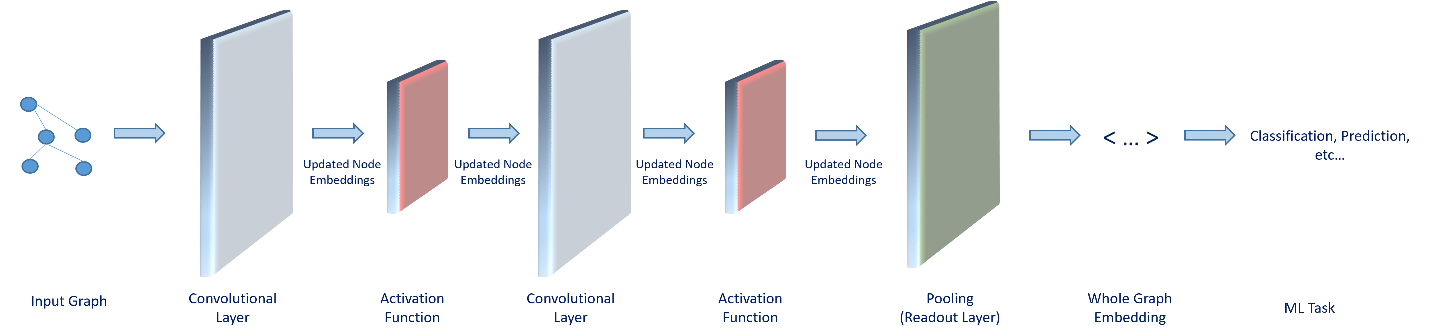
\includegraphics{gcn_model.png}

}

\caption{\label{fig-gcn-concept}Graph convolutional network conceptual
model. A graph is given as input into the model and passed through a
series of convolutional layers and activation functions that produce
embeddings for each node in the graph. The individual node embeddings
are aggregated together by some pooling operation in a readout layer in
order to produce a whole graph embedding as output that can be used for
structured ML tasks such as classification, regression, or prediction.}

\end{figure}%

Herein, for each family of methods, the approach is described
conceptually, and a short, simple example provided to demonstrate how
these approach could be practically applied for read-across purposes
either for the identification of analogue or to perform an endpoint
prediction.

\section{Methods}\label{methods}

\subsection{WL Subtree Kernel Example}\label{sec-wl}

A read-across example, comprising target substance
2-Amino-4,6-dinitrotoluene (2-ADNT) (CASRN 35572-78-2) and its
structural analogues, was identified from the published EPA Provisional
Peer-Reviewed Toxicity Values (PPRTV) assessments. A PPRTV is defined as
a toxicity value derived for use in the EPA Superfund Program. PPRTVs
are derived after a review of the relevant scientific literature using
established EPA Agency guidance on human health toxicity value
derivations. The objective is to provide support for the hazard and
dose-response assessment pertaining to chronic and subchronic exposures
of substances of concern, to present the major conclusions reached in
the hazard identification and derivation of the PPRTVs, and to
characterize the overall confidence in these conclusions and toxicity
values. Current assessments can be accessed on the U.S. Environmental
Protection Agency's (EPA's) PPRTV website at https://www.epa.gov/pprtv.
In cases where there is a paucity of data to derive a PPRTV for a
specific substance, an analogue approach is applied which permits the
use of data from related substances to calculate a screening value. The
exact procedure is described in more detail in Wang et al
\citep{wang_application_2012}.

Five structural analogues with relevant oral non cancer toxicity values
were identified for the target substance 2-ADNT (see
Table~\ref{tbl-pprtv}). Structures were represented as SMILES. WL
subtree kernels were derived for the set of candidate analogues to
compare their pairwise similarities. Morgan chemical fingerprints
(radius = 3, bitvector = 1024) were also derived from which a Jaccard
index was calculated. This would provide a similarity metric typically
relied upon in analogue searching tools already described. Molecular
graph representations were created using the Python package RDKit
\citep{landrum_rdkit}. The open source Python package GraKeL
\citep{siglidis_grakel_2020} was used to implement the WL subtree
kernel.

The code provided shows how the identifiers and SMILES representations
were compiled and converted into molecular graph representations for
calculation of the WL.

\begin{Shaded}
\begin{Highlighting}[]
\NormalTok{dtxsids }\OperatorTok{=}\NormalTok{ [}\StringTok{\textquotesingle{}2{-}Amino{-}4,6{-}Dinitrotoluene\textquotesingle{}}\NormalTok{,}
\StringTok{\textquotesingle{}2,4,6{-}Trinitrotoluene\textquotesingle{}}\NormalTok{,}
\StringTok{\textquotesingle{}2{-}Methyl{-}5{-}nitroaniline\textquotesingle{}}\NormalTok{,}
\StringTok{\textquotesingle{}Isopropalin\textquotesingle{}}\NormalTok{,}
\StringTok{\textquotesingle{}Pendimethalin\textquotesingle{}}\NormalTok{,}
\StringTok{\textquotesingle{}Trifluralin\textquotesingle{}}
\NormalTok{]}

\NormalTok{smiles }\OperatorTok{=}\NormalTok{ [}\StringTok{\textquotesingle{}CC1=C(C=C(C=C1N)[N+]([O{-}])=O)[N+]([O{-}])=O\textquotesingle{}}\NormalTok{,}
\StringTok{\textquotesingle{}CC1=C(C=C(C=C1[N+]([O{-}])=O)[N+]([O{-}])=O)[N+]([O{-}])=O\textquotesingle{}}\NormalTok{,}
\StringTok{\textquotesingle{}CC1=C(N)C=C(C=C1)[N+]([O{-}])=O\textquotesingle{}}\NormalTok{,}
\StringTok{\textquotesingle{}CCCN(CCC)C1=C(C=C(C=C1[N+]([O{-}])=O)C(C)C)[N+]([O{-}])=O\textquotesingle{}}\NormalTok{,}
\StringTok{\textquotesingle{}CCC(CC)NC1=C(C=C(C)C(C)=C1[N+]([O{-}])=O)[N+]([O{-}])=O\textquotesingle{}}\NormalTok{,}
\StringTok{\textquotesingle{}CCCN(CCC)C1=C(C=C(C=C1[N+]([O{-}])=O)C(F)(F)F)[N+]([O{-}])=O\textquotesingle{}}\NormalTok{,}

\NormalTok{]}
\end{Highlighting}
\end{Shaded}

\begin{Shaded}
\begin{Highlighting}[]
\KeywordTok{def}\NormalTok{ smile\_to\_mol\_graph(smile):}

\NormalTok{    mol }\OperatorTok{=}\NormalTok{ Chem.MolFromSmiles(smile)}
\NormalTok{    g }\OperatorTok{=}\NormalTok{ nx.Graph()}

    \ControlFlowTok{for}\NormalTok{ atom }\KeywordTok{in}\NormalTok{ mol.GetAtoms():}
\NormalTok{        g.add\_node(atom.GetIdx(),}
\NormalTok{                   atom\_symbol }\OperatorTok{=}\NormalTok{ atom.GetSymbol())}
    \CommentTok{\# Add edges with bond properties}
    \ControlFlowTok{for}\NormalTok{ bond }\KeywordTok{in}\NormalTok{ mol.GetBonds():}
\NormalTok{        g.add\_edge(bond.GetBeginAtomIdx(), }
\NormalTok{                   bond.GetEndAtomIdx(), }
\NormalTok{                   bond\_type}\OperatorTok{=}\BuiltInTok{str}\NormalTok{(bond.GetBondType()))}

    
    \ControlFlowTok{return}\NormalTok{ g}
\end{Highlighting}
\end{Shaded}

\begin{Shaded}
\begin{Highlighting}[]
\NormalTok{graphs }\OperatorTok{=}\NormalTok{ [smile\_to\_mol\_graph(smile) }\ControlFlowTok{for}\NormalTok{ smile }\KeywordTok{in}\NormalTok{ smiles]}
\NormalTok{grakel\_graphs }\OperatorTok{=}\NormalTok{ grakel.graph\_from\_networkx(graphs,node\_labels\_tag}\OperatorTok{=}\StringTok{\textquotesingle{}atom\_symbol\textquotesingle{}}\NormalTok{)}
\end{Highlighting}
\end{Shaded}

\begin{Shaded}
\begin{Highlighting}[]
\NormalTok{wl\_kernel }\OperatorTok{=}\NormalTok{ grakel.WeisfeilerLehman(base\_graph\_kernel}\OperatorTok{=}\NormalTok{grakel.VertexHistogram,normalize}\OperatorTok{=}\VariableTok{True}\NormalTok{)}
\NormalTok{p }\OperatorTok{=}\NormalTok{ wl\_kernel.fit\_transform(grakel\_graphs)}
\NormalTok{df }\OperatorTok{=}\NormalTok{ pd.DataFrame(p)}
\NormalTok{df.index }\OperatorTok{=}\NormalTok{ dtxsids}
\NormalTok{df.columns }\OperatorTok{=}\NormalTok{ dtxsids}
\end{Highlighting}
\end{Shaded}

\subsection{Node Embedding Example}\label{sec-node2vec}

A dataset of 82 read-across case examples compiled from the literature
taken from Patlewicz et al, \emph{in preparation} was used to explore
the uility of Node2Vec embeddings in comparing analogue pairs. The 82
cases comprised 468 substances which were converted to graph objects as
described in Section~\ref{sec-wl}. The Node2Vec python library was used
to learn node embeddings by creating biased random walks of the
molecular graphs. The embedding dimensions were set to 64, with a random
walk length of 30 and parameters to adjust the balance between
structural equivalence and homophily.

\subsection{Graph Embedding Example}\label{sec-graph2vec}

To demonstrate the applicability of graph embedding methodologies within
a RAx context, an example was developed using a dataset of substances
with associated genotoxicity outcomes. The dataset was an updated
version of that compiled in Pradeep et al
\citep{pradeep_evaluation_2021} drawn from the EPA Toxicity Values
database (ToxValDB). The same methodology as described in Pradeep et al
\citep{pradeep_evaluation_2021} was used to create a dataset with a
summary genotoxicity outcome for each chemical. Genotoxicity studies,
including \emph{in vitro} and \emph{in vivo} chromosomal aberration,
Ames, micronucleus, mouse lymphoma studies were initially retrieved from
ToxValDB. To create a single outcome per chemical, the dataset was first
grouped by substance identifier and summarized as follows: if a
substance was associated with a positive Ames result, a positive
genotoxicity outcome was returned, if a substance was not associated
with a positive Ames but did have a reported positive chromosomal or
micronucleus outcome, it was tagged as a clastogen. If only inconclusive
studies were associated with a substance, an inconclusive tag was
assigned, finally if only negative outcomes were associated with the
substance, a non-genotoxicity outcome was returned. For the dataset
compiled with structural information, there were 5403 chemicals with
QSAR-READY SMILES and a genotoxicity outcome.

Genotoxicity is an endpoint of particular interest where many different
prediction models have been developed from quantitative structure
activity relationships (QSARs) to read-across approaches. Examples of
models include the Ames mutagenicity model that exists within the EPA
TEST suite (see
{[}https://www.epa.gov/comptox-tools/toxicity-estimation-software-tool-test{]}
as well as a myriad of genotoxicity models available within the VEGA
suite of tools (see
{[}https://www.vegahub.eu/portfolio-item/vega-qsar/{]}. Benigni reviewed
the state of the art of modelling genotoxicity
\citep{benigni_data-based_2019} discussing the different approaches that
have been applied to which test guidelines have been modelled. There has
been a renewed interest in building new models for genotoxicity since
the International Conference on Harmonization (ICH) M7 guideline
permited the use of \emph{in silico} approaches for predicting Ames
mutagenicity for the initial assessment of impurities in
pharmaceuticals. The guideline allows for a knowledge base and
statistical model to be used in combination to predict Ames
mutagenicity. Two modelling challenges were established recently to
crowdsource the development of new models to predict the Ames
mutagenicity, first of which was reported in Honma et al
\citep{honma_improvement_2019} with a followup study described in
Furuhama et al. \citep{Furuhama_2023}.

Beyond QSAR approaches, read-across approaches have been also been
applied to genotoxicity as discussed by Benigni
\citep{benigni_towards_2019}. One quantitative read-across approach
includes the method employed by GenRA \citep{shah_systematically_2016},
wherein structural aspects of chemicals are used in a K
nearest-neighbors (k-nn) classification to derive a similarity weighted
activity outcome. Morgan chemical fingerprints form one possible set of
structural features to identify similar substances to perform a
read-across. An alternative approach is to employ graph representations
and embedding methods such as Graph2Vec, GL2Vec, and LDP to characterize
substances and identify analogues. Herein, the constructed dataset was
used to perform a genotoxicity prediction where the three aforementioned
methods were used to create molecular graph representations as a basis
to identify similar analogues.

Molecular graph representations were generated using the open source
Python package RDKit as described in Section~\ref{sec-wl}. Graph2Vec,
GL2Vec, and LDP embedding models, implemented within the Python package
KarateClub \citep{karateclub}, were used to generate vectorized
embeddings for each substance. The embeddings were projected in 2D using
a t-distributed stochastic neighborhood embedding (t-SNE)
\citep{van_er_maaten_visualizing_2018}, which was color coded by
genotoxicity outcome. The embeddings were used as inputs in 2
classifiers; a k-nn classifier and logistic regression to assess their
informative content. As a baseline comparator, Morgan chemical
fingerprints were used as feature inputs into the same two classifiers.
The 2 classifiers were implemented using the open source Python package
scikit-learn \citep{RN53} with the area under the curve-receiver
operating characteristic (AUC-ROC) as a performance metric.

\subsection{GCN Embeddings Example}\label{gcn-embeddings-example}

The same dataset as described Section~\ref{sec-graph2vec} was used to
demonstrate the applicability of the GCN embedding method within a RAx
context. An end-to-end GCN supervised graph classification model was
constructed by using three convolutional layers (GATv2Conv convolutional
layer, a graph attentional layer from Brody et al., \citep{RN56}) with
ReLU activation functions, a global mean pooling readout layer, and a
single fully connected linear layer to make predictions. For the
molecular graphs, one hot encodings of the atom symbol labels were
attached as node feature vectors. The graphs were split into a training
and validation set of size 4,000 and 1,403 respectively. Using cross
entropy loss and an Adam optimizer with a learning rate of 0.001, the
model was trained over 50 epochs, with the AUC score of the training and
validation graphs reported at each epoch. After training, embeddings for
the validation graphs were generated by inputting the graphs into the
trained model and extracting the resultant embedding from the readout
layer. These were visualized via t-SNE and labeled by outcome. The
embeddings were also used as inputs into k-nn and logistic regression
classification models, with performance compared against the use of
Morgan chemical fingerprints.

\section{Results}\label{results}

\subsection{WL Subtree Kernel}\label{wl-subtree-kernel}

Based on an expert-driven evaluation of the structural, physicochemical,
available toxicokinetic (TK) data, and toxicity data,
2,4,6-Trinitrotoluene (TNT) was chosen as the `best analogue' primarily
based on its metabolic similarity, structural similarity, and shared
metabolites. The similarity of toxicological outcomes across all the
source analogues established confidence in the toxicologic read-across
for 2-ADNT. TNT was also determined to be the most health-protective
analogue because its point of departure (POD) and corresponding
reference dose (RfD) value were lower than the other candidate
analogues. WL and Jaccard (based on Morgan fingerprints) pairwise
similarities across the target and all analogues are shown in
Figure~\ref{fig-timeline}. TNT had both the highest WL and Jaccard
score. The Jaccard similarities based on Morgan fingerprints were
notably lower from the WL scores though the ranking in terms of the
similarities relative to the target chemical was largely comparable. The
difference between nitro group vs.~amino group accounted for the slight
decrease in WL score from the target 2-ADNT whereas the position of the
methyl group appeared not to impact the score. The remaining candidate
analogues all had lower WL scores owing to the change of substituent
position as well as the substituents themselves. The high WL scores are
likely to be as a result of the manner in which the graph was initially
constructed using only atom symbols as labels. The absence of other
relevant atom properties might better discriminate the differences
between the analogues. Substances with similar overall topology but
different substituents are likely to yield high WL scores since the WL
kernel is sensitive to the global structure of the chemical and may
overemphasize this at the expense of distinct local features. To explore
this further the manner in which the graphs were constructed (see
related code) was refined to incorporate additional atom property
information and the WL scores were re-computed.

\begin{figure}

\begin{minipage}{0.50\linewidth}

\begin{figure}[H]

\centering{

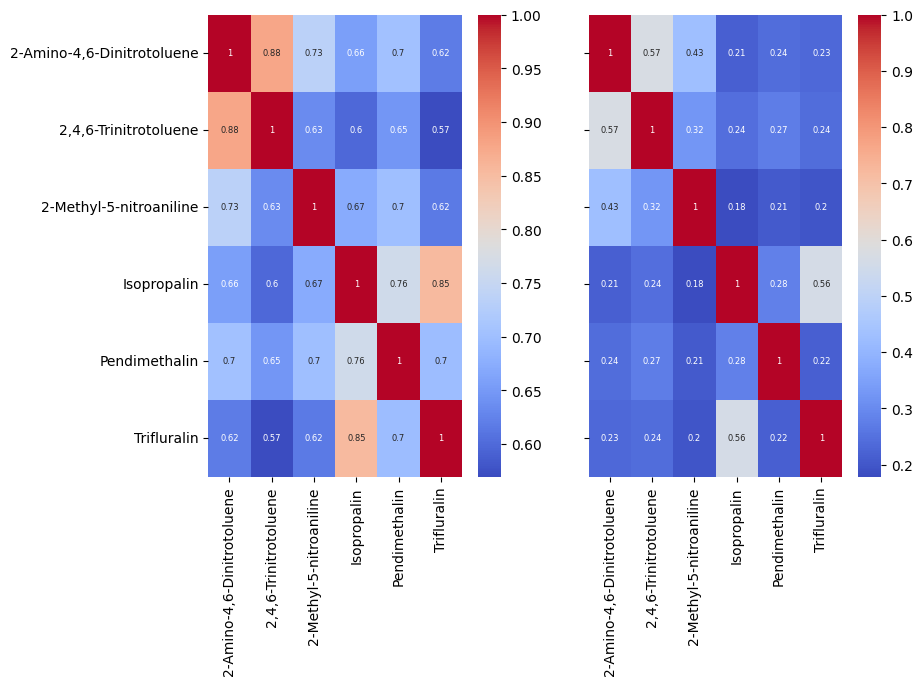
\includegraphics{survey_files/figure-pdf/fig-timeline-output-1.png}

}

\caption{\label{fig-timeline}Pairwise similarities based on WL and
Jaccard Morgan Fingerprints}

\end{figure}%

\end{minipage}%

\end{figure}%

\begin{Shaded}
\begin{Highlighting}[]
\KeywordTok{def}\NormalTok{ smile\_to\_mol\_graph(smile):}
\NormalTok{    mol }\OperatorTok{=}\NormalTok{ Chem.MolFromSmiles(smile)}
\NormalTok{    g }\OperatorTok{=}\NormalTok{ nx.Graph()}
    
    \CommentTok{\# Add nodes with atom properties}
    \ControlFlowTok{for}\NormalTok{ atom }\KeywordTok{in}\NormalTok{ mol.GetAtoms():}
\NormalTok{        node\_label }\OperatorTok{=} \SpecialStringTok{f"}\SpecialCharTok{\{}\NormalTok{atom}\SpecialCharTok{.}\NormalTok{GetSymbol()}\SpecialCharTok{\}}\SpecialStringTok{\_}\SpecialCharTok{\{}\NormalTok{atom}\SpecialCharTok{.}\NormalTok{GetDegree()}\SpecialCharTok{\}}\SpecialStringTok{\_}\SpecialCharTok{\{}\BuiltInTok{str}\NormalTok{(atom.GetHybridization())}\SpecialCharTok{\}}\SpecialStringTok{\_}\SpecialCharTok{\{}\NormalTok{atom}\SpecialCharTok{.}\NormalTok{GetIsAromatic()}\SpecialCharTok{\}}\SpecialStringTok{"}
\NormalTok{        g.add\_node(atom.GetIdx(), }
\NormalTok{                   atom\_label}\OperatorTok{=}\NormalTok{node\_label)}

    \CommentTok{\# Add edges with bond properties}
    \ControlFlowTok{for}\NormalTok{ bond }\KeywordTok{in}\NormalTok{ mol.GetBonds():}
\NormalTok{        g.add\_edge(bond.GetBeginAtomIdx(), }
\NormalTok{                   bond.GetEndAtomIdx(), }
\NormalTok{                   bond\_type}\OperatorTok{=}\BuiltInTok{str}\NormalTok{(bond.GetBondType()))}

    \ControlFlowTok{return}\NormalTok{ g}
\end{Highlighting}
\end{Shaded}

Table~\ref{tbl-pprtv} compares the refined WL scores with the original
WL based on atom labels alone and the Jaccard metric. Whilst the naive
WL scores gave rise to the highest scores, incorporating additional atom
property information (including aromaticity, hybridization and atom
degree) refines the score (WL-rev) so that the differences between the
substituents and their positions are better accounted for. The WL scores
offer an effective means of computing a similar score direct from the
structural representation bypassing the need to compute separate
chemical fingerprints or descriptors. The approach was sensitive to the
manner in which the graphs were constructed and care needs to be placed
on incorporating atom and bond information so that small local
differences between substances such as substituent differences on an
aromatic ring structure are not lost in the manner in which global
structure is characterized. Careful consideration of the type of
information to attribute through label selection is an important aspect
of this graph kernel operation.

\begin{longtable}[]{@{}cccccc@{}}
\caption{2-ADNT is denoted as the target substance based on its role
designation. TNT was ultimately selected as the read-across candidate
out of the 5 candidate analogues. WL, Jaccard and WL-rev denote the
similarity scores computed. WL relies on molecular graphs constructed
using only atoms as labels whereas WL-rev scores were derived taking
into account other atom property information. The pairwise scores are
shown in each case. e.g.~TNT was determined to have a Jaccard similarity
with 2-ADNT of 0.57 whereas the WL score and revised WL score was 0.88
and 0.73 respectively.}\label{tbl-pprtv}\tabularnewline
\toprule\noalign{}
Substance & Role & DTXSID & WL & Jaccard Morgan FP & WL-rev \\
\midrule\noalign{}
\endfirsthead
\toprule\noalign{}
Substance & Role & DTXSID & WL & Jaccard Morgan FP & WL-rev \\
\midrule\noalign{}
\endhead
\bottomrule\noalign{}
\endlastfoot
2-ADNT & Target & DTXSID6044068 & 1 & 1 & 1 \\
TNT & Selected & DTXSID7024372 & 0.88 & 0.57 & 0.73 \\
2-Methyl-5-nitroaniline & Candidate & DTXSID4020959 & 0.73 & 0.43 &
0.52 \\
Isopropalin & Candidate & DTXSID8024157 & 0.66 & 0.21 & 0.45 \\
Pendimethalin & Candidate & DTXSID7024245 & 0.70 & 0.24 & 0.50 \\
Trifluralin & Candidate & DTXSID4021395 & 0.62 & 0.23 & 0.42 \\
\end{longtable}

\subsection{Node Embedding}\label{node-embedding}

The cosine distance for selected read-across examples (see
Table~\ref{tbl-icf}) were calculated on the basis of the node
embeddings. On first inspection, the node embeddings appear promising
given the low cosine distances - the read-across candidates were found
to be similar to their respective targets. However the maximum cosine
distance across the overall dataset was determined to be quite low
(0.44). Indeed, the pairwise cosine distances based on the embeddings
for two random chemicals extracted from the dataset, chlorobenzene and
caffeine was computed to be 0.19 which is not that much higher than for
their respective candidate analogues. A permutation test between all the
individual read-across cases relative to the overall dataset found that
67\% of case examples had maximum pairwise distances that were not
significantly different. Overall the node embeddings produced did not
appear to be able to discriminate read-across case substances that were
considered to be particularly similar in terms of their structure
relative to the entire dataset suggesting other embeddings that are able
to capture the whole graph might be more promising.

\begin{longtable}[]{@{}cccccc@{}}
\caption{Selected targets and their candidate analogues and their
corresponding pairwise cosine scores.}\label{tbl-icf}\tabularnewline
\toprule\noalign{}
Substance & Role & DTXSID & Cosine Distance & & \\
\midrule\noalign{}
\endfirsthead
\toprule\noalign{}
Substance & Role & DTXSID & Cosine Distance & & \\
\midrule\noalign{}
\endhead
\bottomrule\noalign{}
\endlastfoot
Chlorobenzene & Target & DTXSID4020298 & 0 & & \\
1,4-Dichlorobenzene & Candidate & DTXSID1020431 & 0.12 & & \\
1,2-Dichlorobenzene & Candidate & DTXSID6020430 & 0.14 & & \\
Caffeine & Target & DTXSID0020232 & 0 & & \\
Theophylline & Candidate & DTXSID5021336 & 0.14 & & \\
Theobromine & Candidate & DTXSID9026132 & 0.11 & & \\
\end{longtable}

\subsection{Graph Embedding}\label{graph-embedding}

Figure~\ref{fig-graph2vec}, Figure~\ref{fig-gl2vec} and
Figure~\ref{fig-ldp} show the embeddings for Graph2Vec, GL2Vec and LDP
as projected into t-SNE plot and color coded by genotoxicity outcome.
The mean AUC-ROC scores from 5-fold cross validation classifiers are
shown in Table~\ref{tbl-graph2vec}.

\begin{figure}[H]

\centering{

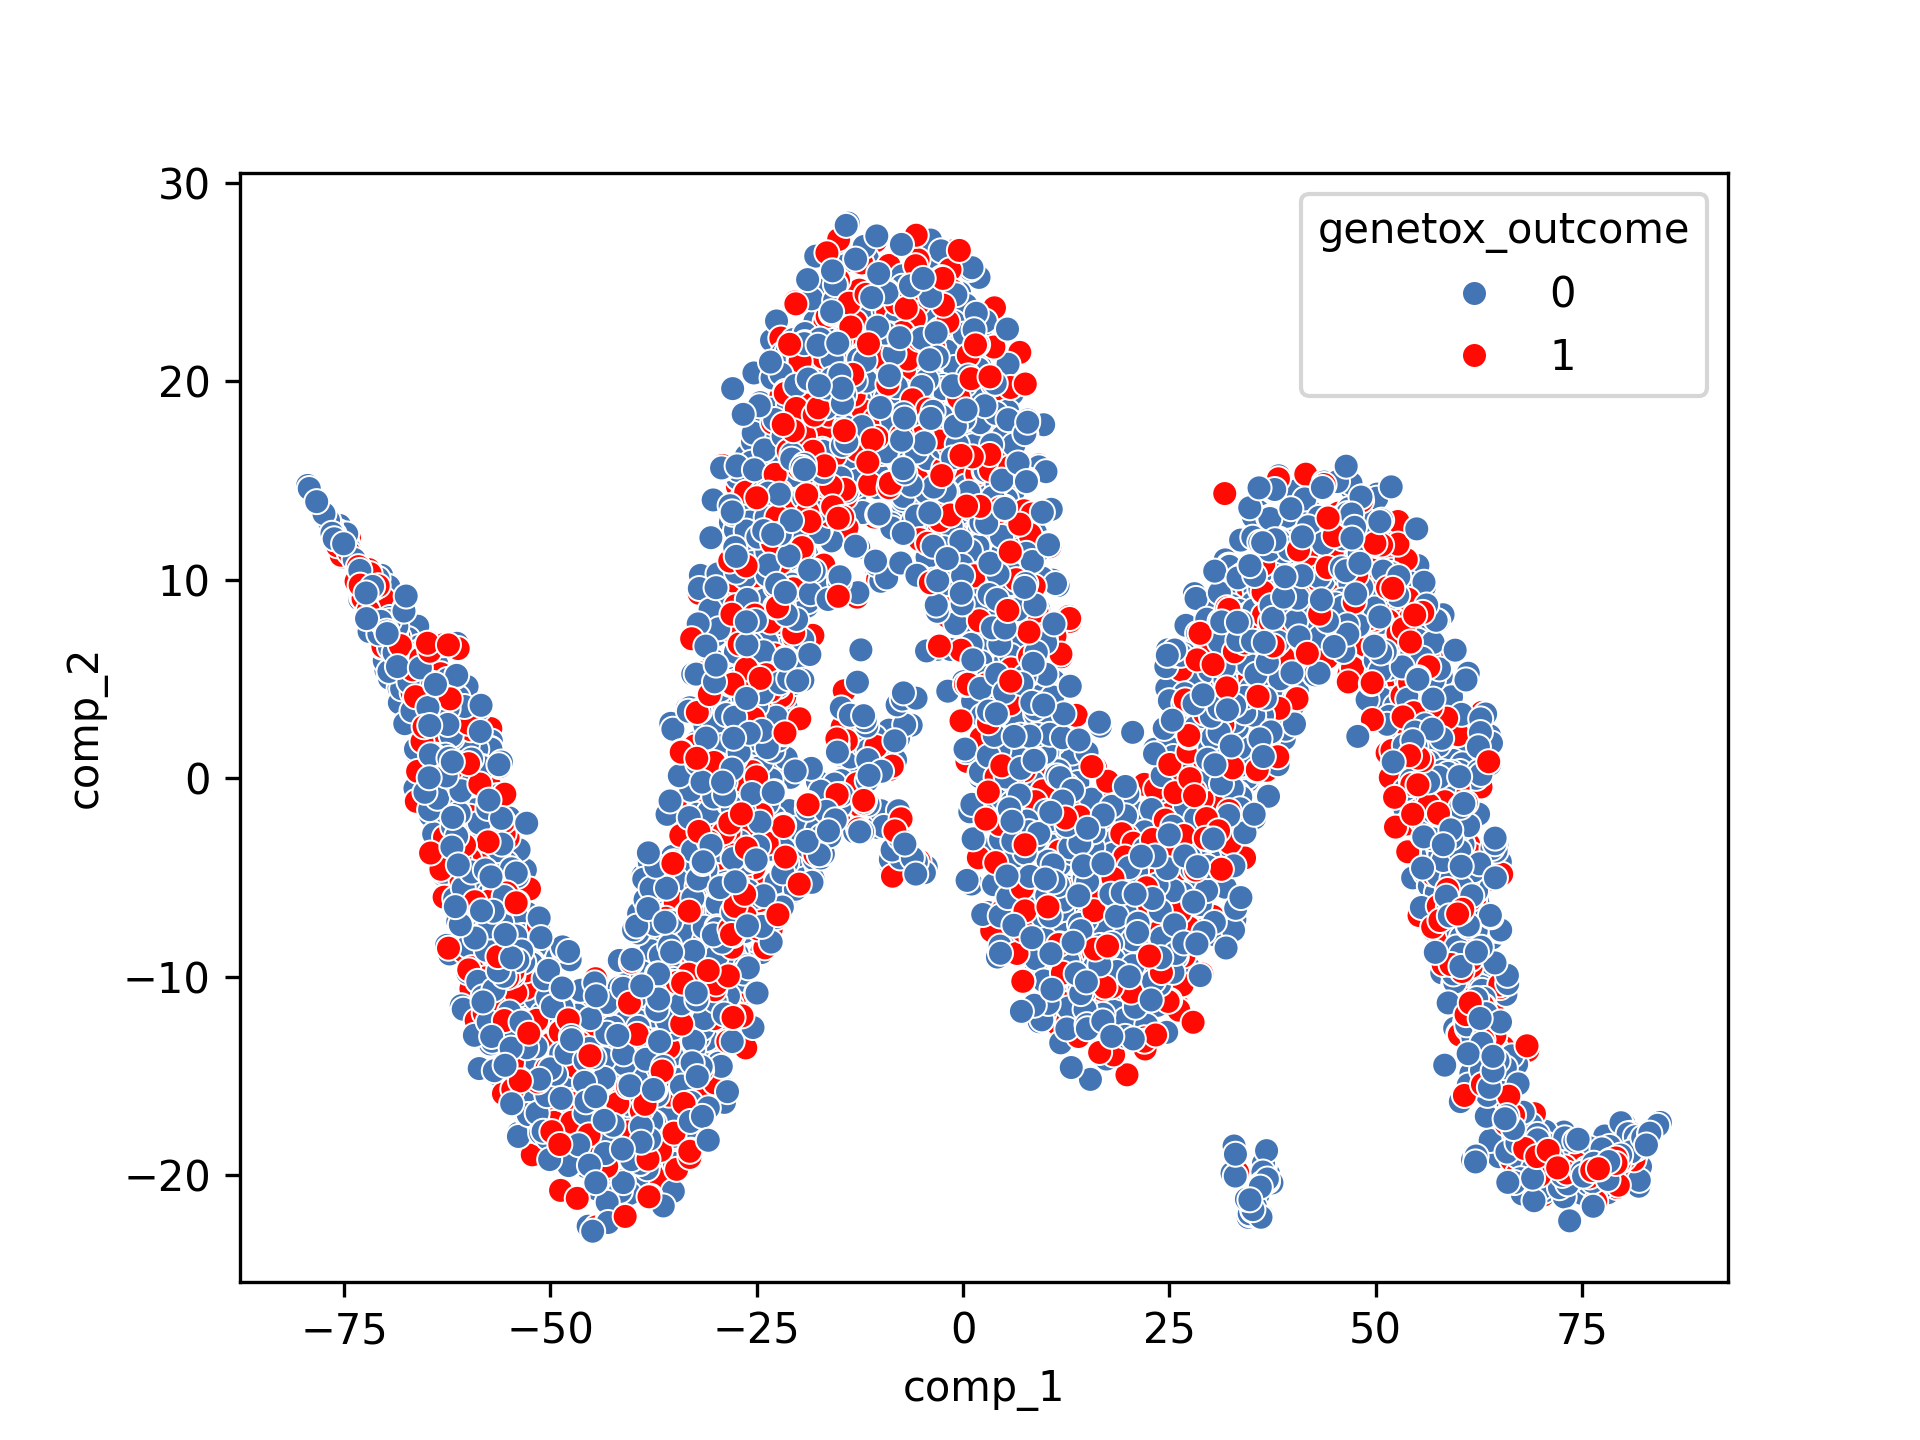
\includegraphics[width=0.5\textwidth,height=\textheight]{Graph2Vec_250724.png}

}

\caption{\label{fig-graph2vec}Graph2Vec embeddings labeled by
genotoxicity outcome}

\end{figure}%

\begin{figure}[H]

\centering{

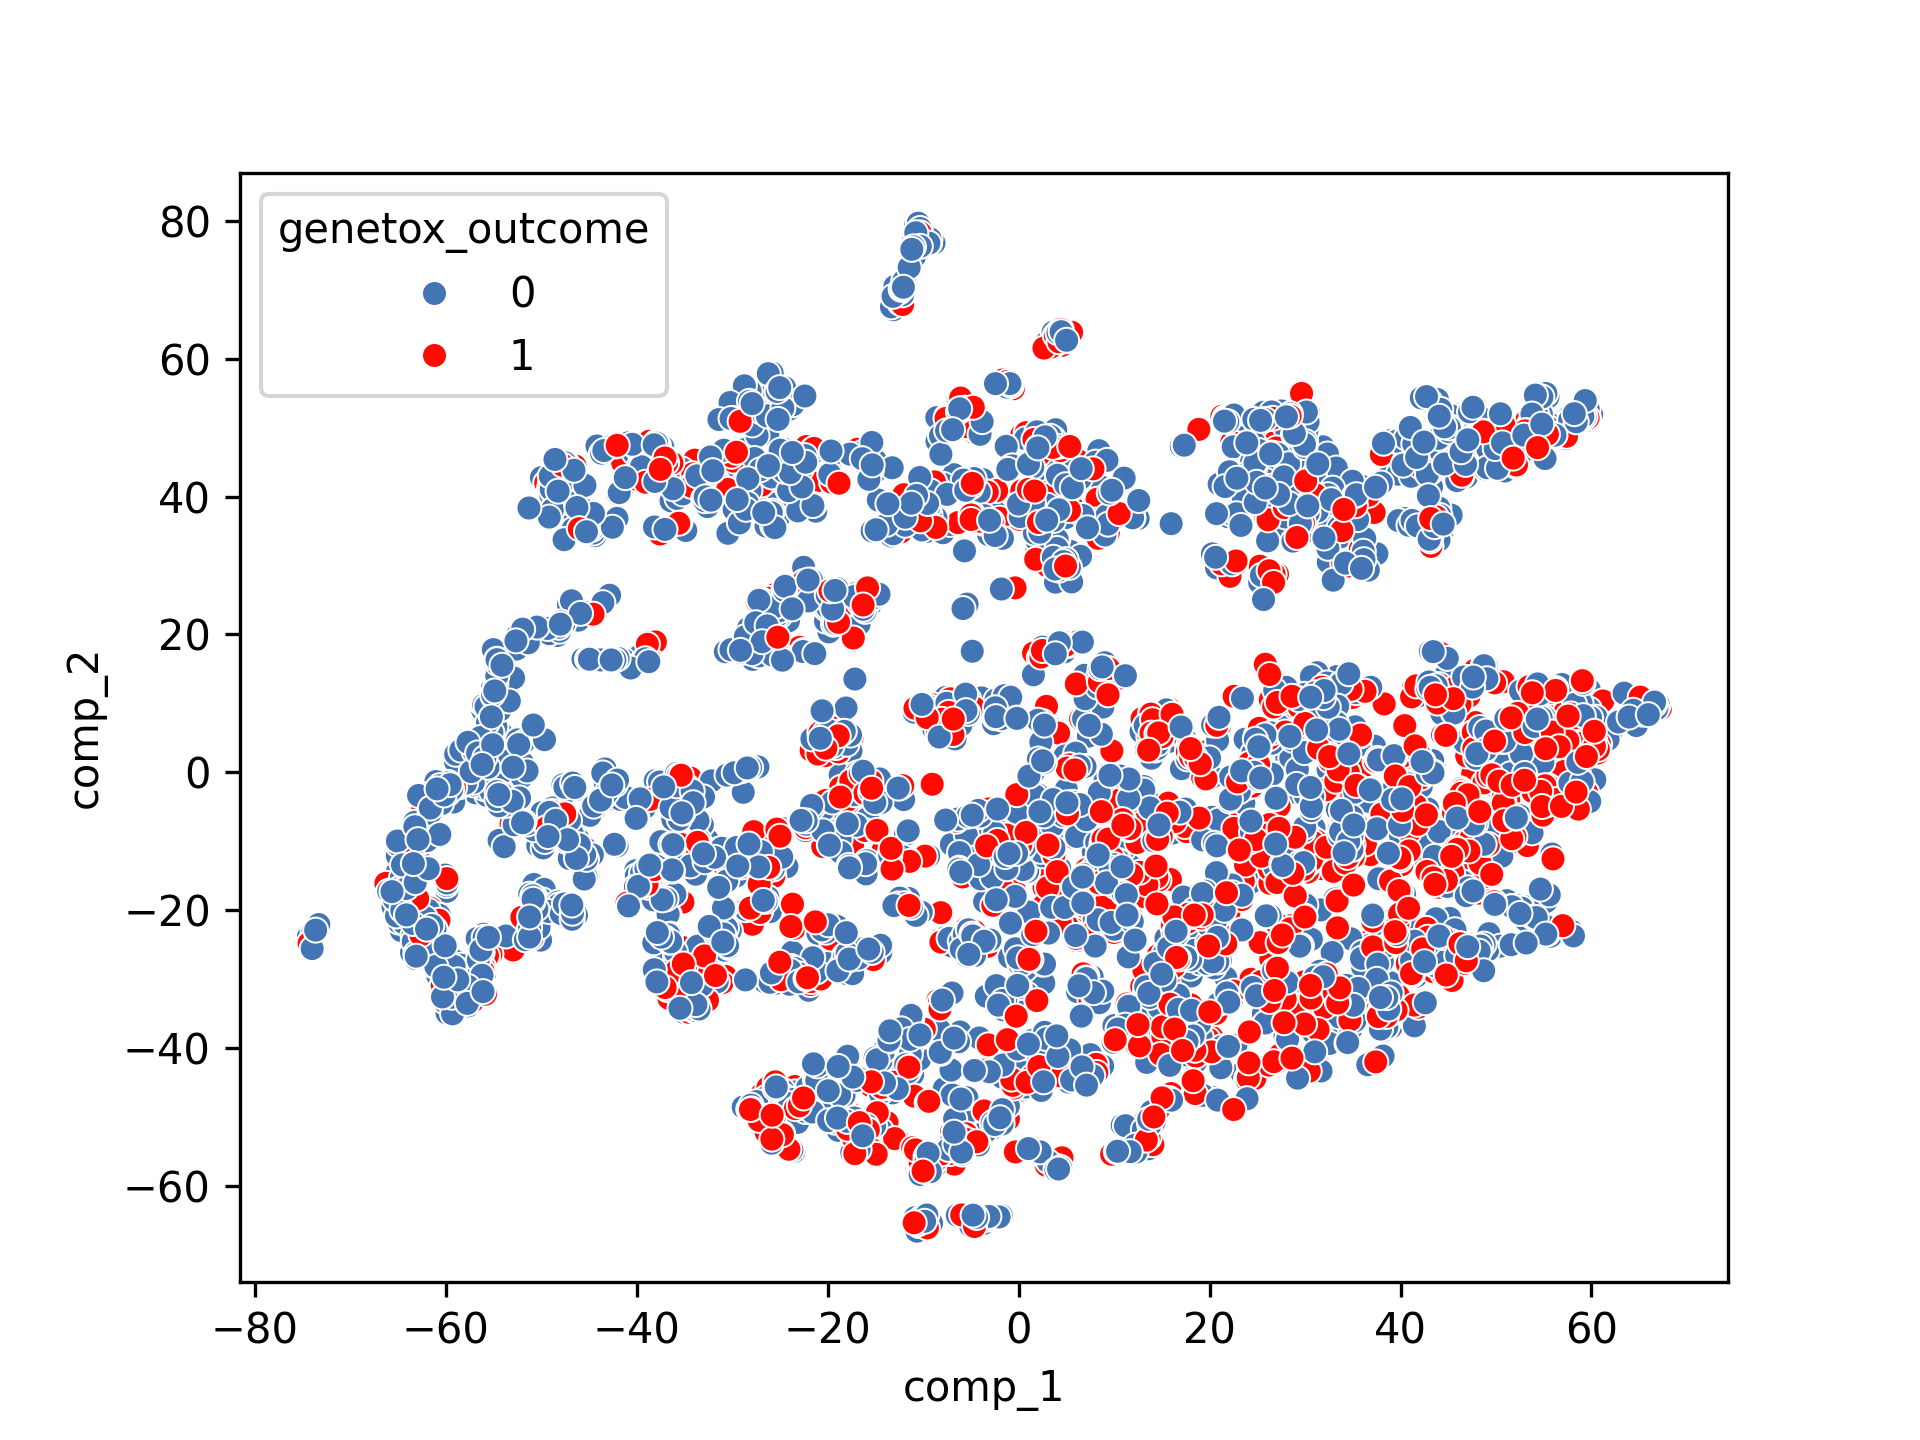
\includegraphics[width=0.5\textwidth,height=\textheight]{GL2Vec_250724.png}

}

\caption{\label{fig-gl2vec}GL2Vec embeddings labeled by genotoxicity
outcome}

\end{figure}%

\begin{figure}[H]

\centering{

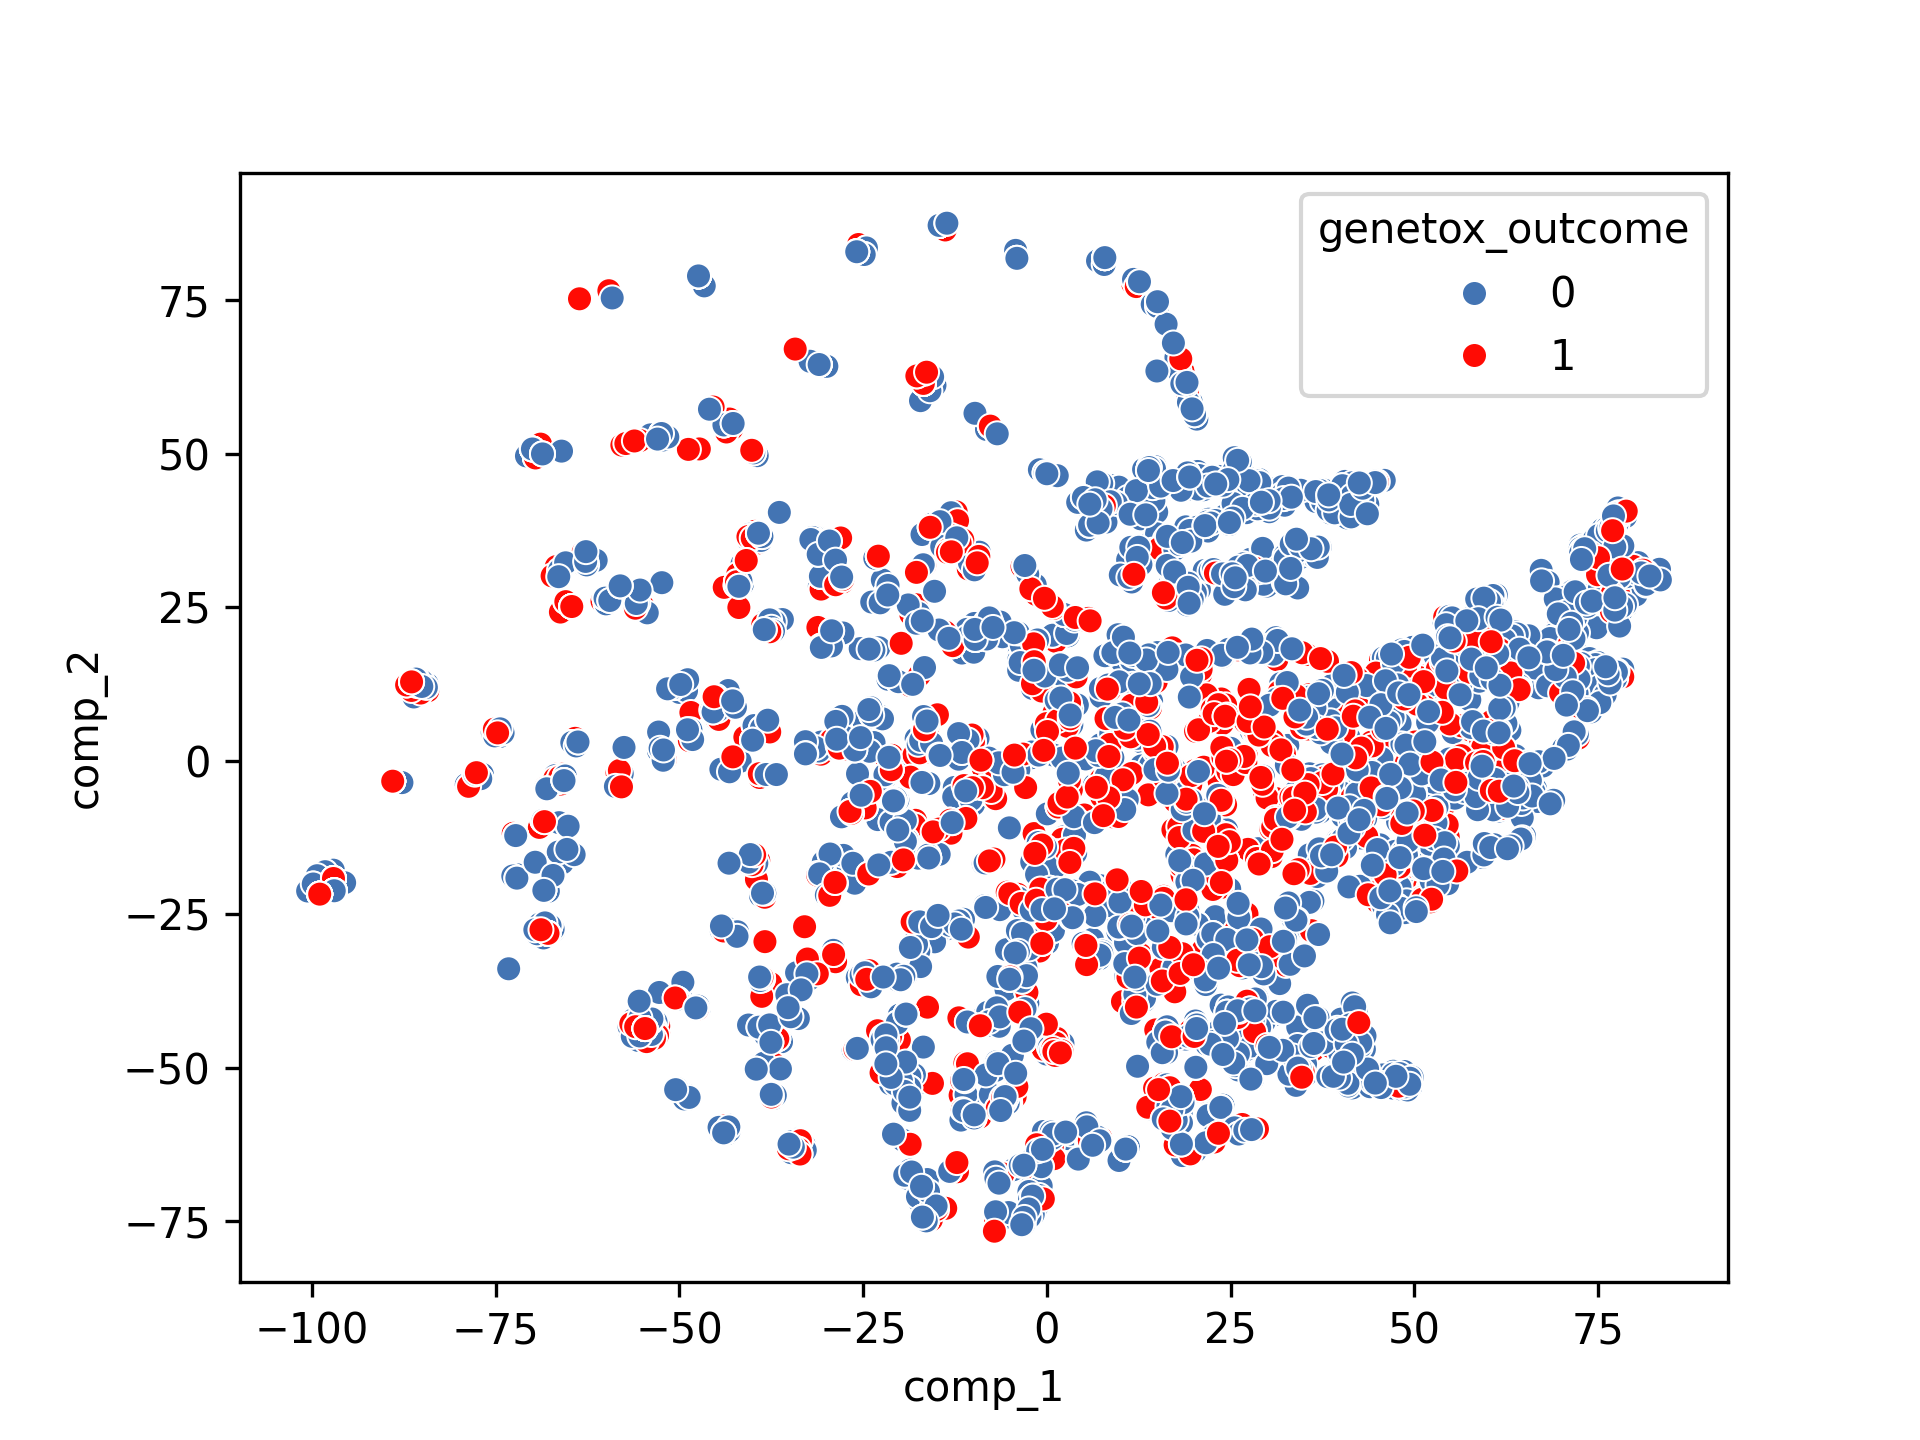
\includegraphics[width=0.5\textwidth,height=\textheight]{LDP_250724.png}

}

\caption{\label{fig-ldp}LDP embeddings labeled by genotoxicity outcome}

\end{figure}%

\begin{longtable}[]{@{}ccc@{}}
\caption{5-fold cross validated k-nn and logistic regression
genotoxicity classification results using Morgan fingerprints and the
three embeddings methods .}\label{tbl-graph2vec}\tabularnewline
\toprule\noalign{}
Embedding Method & K-nn & Logistic Regression \\
\midrule\noalign{}
\endfirsthead
\toprule\noalign{}
Embedding Method & K-nn & Logistic Regression \\
\midrule\noalign{}
\endhead
\bottomrule\noalign{}
\endlastfoot
Morgan FPs & 0.662 & 0.727 \\
Graph2Vec & 0.526 & 0.500 \\
GL2Vec & 0.604 & 0.598 \\
LDP & 0.596 & 0.549 \\
\end{longtable}

The quality of the embeddings generated by Graph2Vec, GL2Vec, or LDP
failed to capture relevant chemical features effectively to be able to
discriminate between genotoxic and non-genotoxic outcomes. Morgan
chemical fingerprints outperformed the graph embeddings using both
classifiers. Graph2Vec struggled to separate the data, with almost no
discrimination between the two outcomes as shown in
Figure~\ref{fig-graph2vec}. GL2Vec and LDP both provided better
discrimination, with clearer clustering of genotoxic and non-genotoxic
chemicals (Figure~\ref{fig-gl2vec} and Figure~\ref{fig-ldp}). Fine
tuning parameters such as embedding length and learning rates may
increase performance since all embeddings were generated using the
default parameters of the models. Default parameters were also used for
the classification models, leaving another area of possible improvement.
The graph representations used were also very simple, using only the
atom symbol as the node labels. Different types of labels may lead to
better performance in embedding methods that rely on node label
information alone.

\subsection{GCN Embeddings}\label{gcn-embeddings}

GCN embeddings were visualized via t-SNE and labeled by outcome as shown
in Figure~\ref{fig-gcn-nn}. The 5-fold cross validation AUC scores for
the K-nn and Logistic regression using the GCN embeddings were found to
be 0.66 and 0.78 repectively, a comparable performance to Morgan
fingerprints using a K-nn approach but a marked improved with the
logistic regression.

\begin{figure}[H]

\centering{

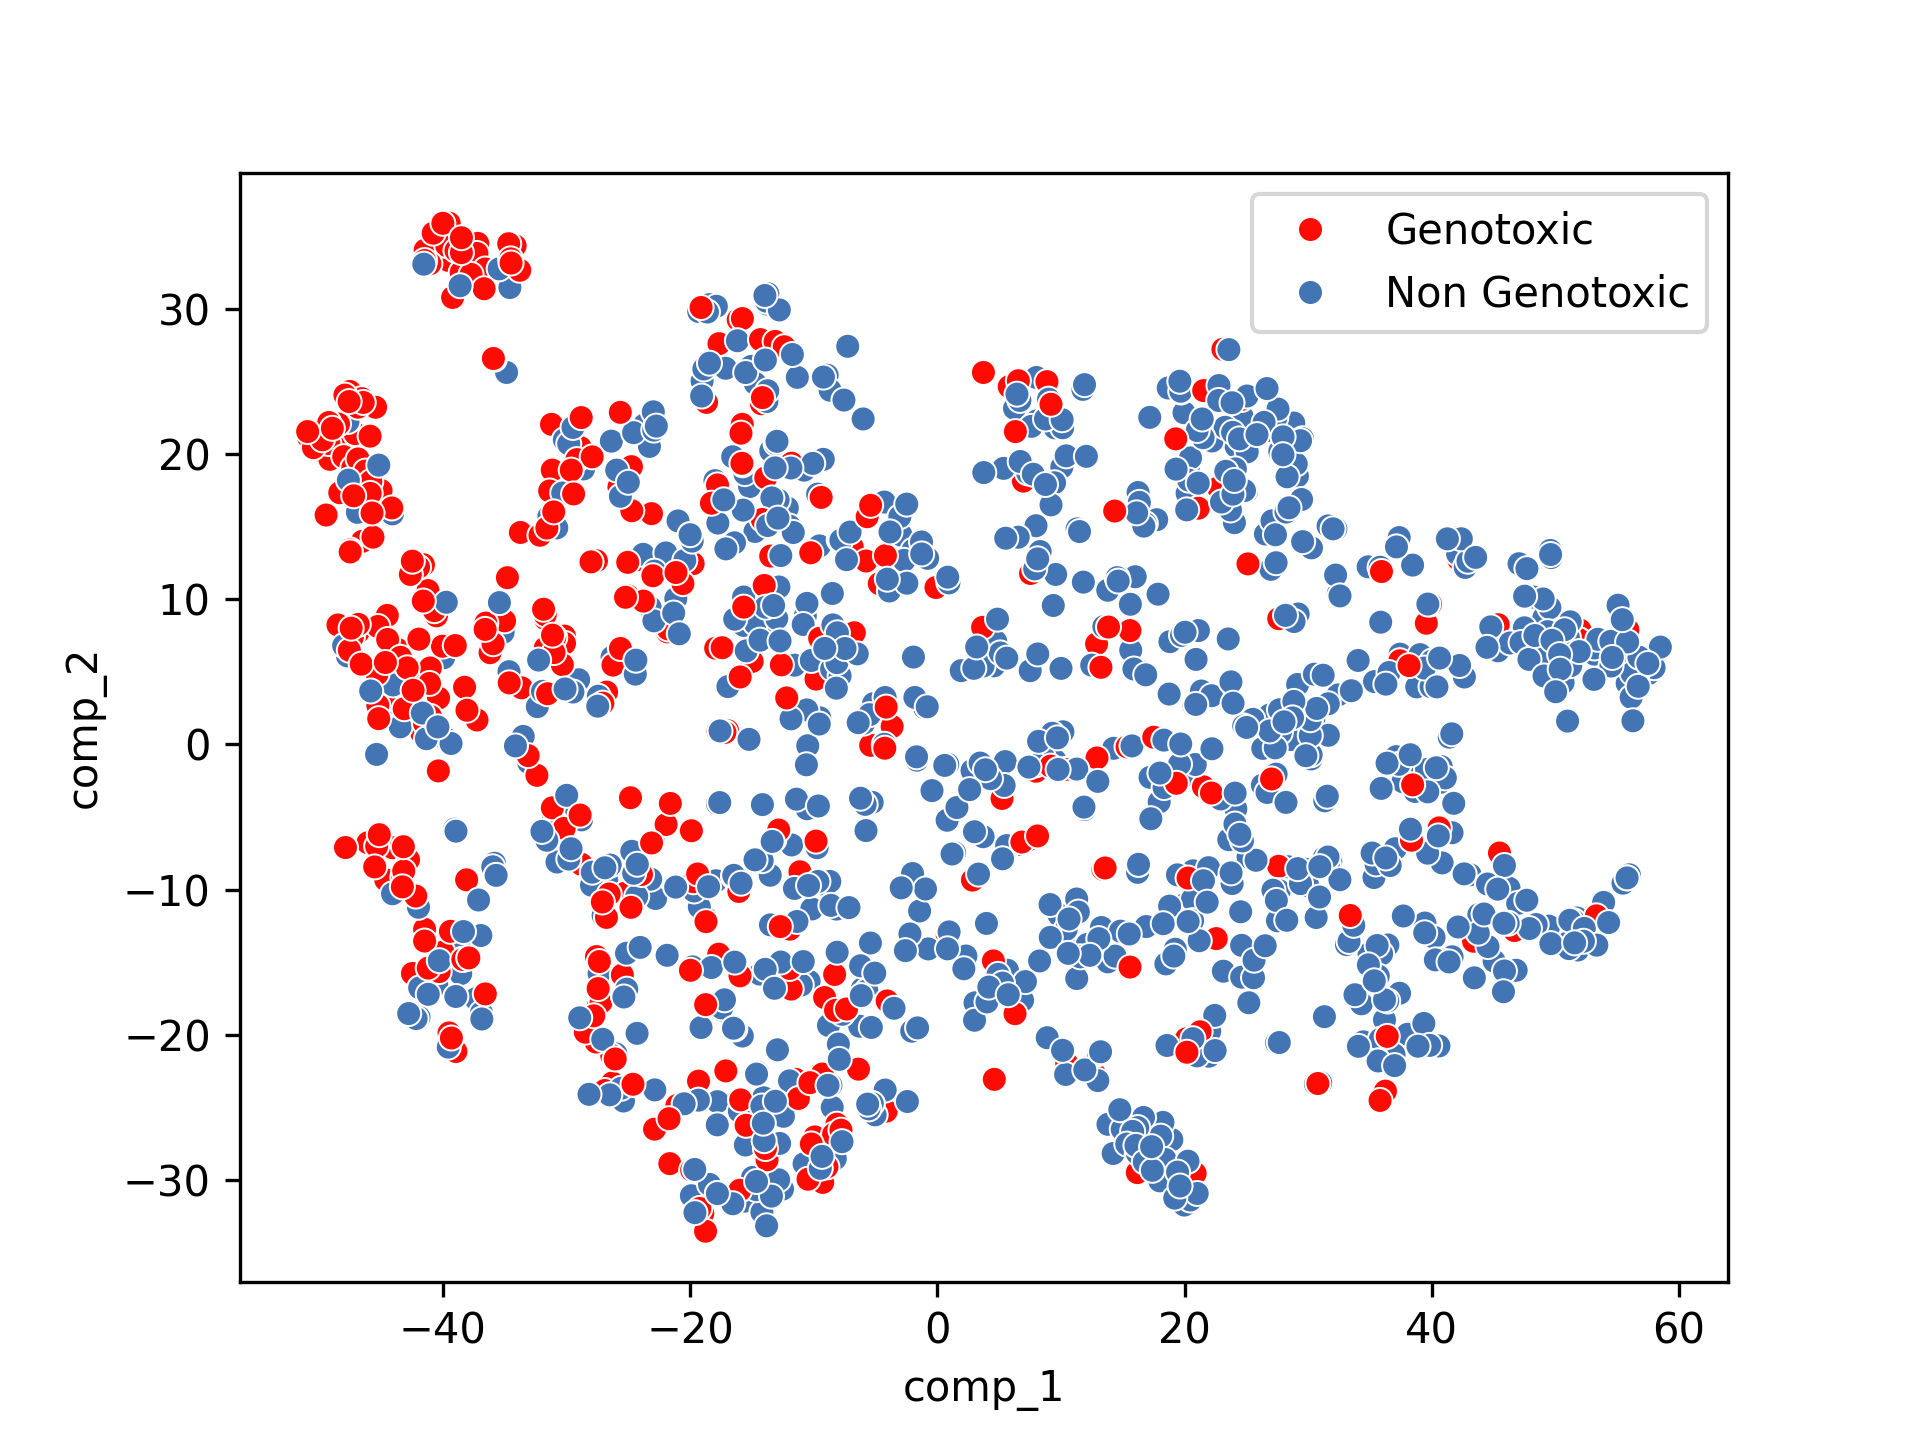
\includegraphics{GCN_embedding_050824.png}

}

\caption{\label{fig-gcn-nn}GCN embeddings of validation graph set
labeled by genotoxicity outcome}

\end{figure}%

A clearer separation between genotoxic and non-genotoxic chemicals in
the embedded space created by the supervised classification GCN model
was observed (Figure~\ref{fig-gcn-nn}) with an improvement in both the
K-nn and logistic regression classification performance relative to
using Morgan fingerprints. As with the previous graph embedding
discussed in Section~\ref{sec-graph2vec}, default parameters were used
for both classification models, likely leaving room for improvement in
performance through hyperparameter tuning. As with all DL models, there
are a large number of options available when constructing a GCN
architecture. Layer types, selection of activation functions, pooling
methods, choice of loss functions and optimizers, as well as the fine
tuning of parameters such as the optimizer's learning rate, the number
of training epochs and number of neurons per layer are all of
significant importance in a network's performance. Further
experimentation with network architecture would likely lead to better
performance, but for the purposes of this illustrative example, the
application of a generically designed network without any fine tuning
was still able to yield reasonable performance.

\section{Conclusion}\label{conclusion}

In this tutorial review, a selection of approaches to quantifying graph
similarity were described and demonstrated for their role in identifying
and evaluating analogues within a read-across approach. A WL graph
kernel approach was found to be useful in characterizing potential
analogues relative to 2-ADNT, identifying TNT as the most similar
analogue. TNT was selected as the source analogue for use in the
read-across assessment. The WL scores were found to be sensitive to the
way in which the graphs were initially constructed such that if atom and
bond characteristics were not sufficiently captured, local differences
in structural representations could be underrepresented relative to the
whole molecular effects and thereby overinflating the resulting scores.
Careful attention is needed to capture node and edge information before
their use. Both the WL with atom labels or a revised WL taking into
account additional atom properties identified TNT as the most similar
analogue to 2-ADNT, their relative ranking of analogues was the same
even though the actual WL scores differed. The Jaccard scores using
Morgan fingerprints were lower no doubt highlighting that small changes
in substituents and their positions are not well discriminated across
the analogues relative to the target substance. Topological and label
information played a significant role in ascertaining the WL
similarities.

In contrast embedding approaches building on the Word2Vec approach were
found to be poor at capturing relevant molecular information and were
ineffective in discriminating between substances that were read-across
candidates (using Node2Vec to learn embeddings) or as in the second
example were categorized as genotoxic or not. In the latter example,
Morgan fingerprints were found to be superior in predicting the
genotoxicity outcomes. Graph2Vec and LDP performed particularly poorly
whereas GL2Vec was slightly better at discriminating genotoxicity or not
using the 2 classifiers.

A Deep learning GCN model fared better, with a marked improvement in
performance compared with Morgan fingerprints. Whereas the embedding
approaches applied in Section~\ref{sec-graphembed} were unsupervised in
nature, the GCN required labeled training data to create informed
embeddings to facilitate genotoxicity classification. This performance
increase observed also came at a cost of resources, and complexity. The
GCN approach can be computationally expensive, depending on model
parameters, scale of datasets, size of graphs and graph features, and
more. These examples illustrate the potential that graph similarity
approaches could play significant roles in the identification of
suitable analogues for RAx However careful attention needs to be paid to
the embedding representation applied and how the initial graphs are
constructed.

\section*{References}\label{references}
\addcontentsline{toc}{section}{References}

\section*{Disclaimer}\label{disclaimer}
\addcontentsline{toc}{section}{Disclaimer}

This manuscript reflects the opinions of the authors and are not
reflective or the opinions or policies of the US EPA.


  \bibliography{bibliography.bib}



\end{document}
